\squarebox[LightBlue]{
\chapterabstract{This chapter reviews the key concepts underlying this thesis, beginning with an overview of low-latency applications and time-varying capacity networks, such as 4G, 5G, and Wi-Fi. Subsequently, the chapter introduces machine learning paradigms and a background on anomaly detection techniques for time series. Finally, it explores root cause diagnosis approaches for cellular and Wi-Fi networks.}
% add that we address xthe limitations in the thesis
}

\minitoc
%\newpage

% \contributions{
% This is an example of a rounded color box with cyan background and black border. 
% You can adjust the color and content as needed.
% }

\section{Low-latency applications}
\ac{LL} applications encompass a diverse range of use cases, including \ac{CG}, \ac{VR}, video conferencing, tele-robotics, industrial automation, and remote surgery. Although these applications share the common requirement of minimal end-to-end delay, each has unique characteristics and demands in terms of latency, throughput, and network protocols. 

Table \ref{tab:ll_applications} provides a summary of LL applications, highlighting their typical uplink and downlink bitrate requirements as well as the range of end-to-end latency values and compare it to video streaming which is non-interactive application.
% remove video streaming
\begin{table*}[!ht]
\setlength\tabcolsep{1pt} 
    
\begin{tabular*}{\linewidth}{@{\extracolsep{\fill}} llll}
    \toprule
       \bf LL & \bf Uplink & \bf Downlink & \bf End-to-end \\
       \bf Application & \bf Bitrate (Mbps) & \bf Bitrate (Mbps) & \bf Latency (ms) \\
    \addlinespace
    \cmidrule{1-4}
    \bf Video streaming & 0.5-3  & 3-25 & $\geq$ 300 (non interactive) \\
    \cmidrule{1-4}
    \bf Video conference & 1-3 & 1-4 & $\leq$ 300 \\
    \bf Cloud Gaming  & 2-5 & 3-40 & $\leq$ 60-100 \\
    \bf Cloud VR & 10 &  25-100 & $\leq$ 20 \\
    \bf Medical surgery & 0.5-10 & 10-100 & $\leq$ 1 \\
    \bottomrule

\end{tabular*}
\caption{Characteristics of Low-latency applications}
\label{tab:ll_applications}
\end{table*}

In this thesis, we focus on Cloud Gaming and Cloud Virtual Reality, two of the most demanding LL applications in terms of bandwidth and latency requirements. Unlike mission-critical applications such as remote medical surgery, CG and Cloud VR have established commercial implementations and deployments, providing a practical foundation for realistic experiments. These applications also represent significant business opportunities for network operators like Orange, as addressing the challenges they present is crucial for enhancing user experience and meeting the growing demand for LL services.
% specifier pourquoi cd et cloud vr avec l'interet pour orange et les challenges (justification)

\subsection{Cloud gaming}

\ac{CG} (sometimes referred to as game streaming) is a gaming paradigm where the player sends its game commands to a server located in the cloud that executes the game and produces video frames that is streamed back to the player. This gaming paradigm implies that powerful computing resources such as \ac{GPU}, are no longer required by gamers as \ac{CG} can be operated on a wide range of devices such as smartphones or thin clients.
\ac{CG} arise with cloud computing and the first commercial cloud gaming platforms were OnLive and Gaikai \cite{onlive, Gaikai}.
Recent years have seen new entrants in the \ac{CG} markets. Sony acquired Gaikai in 2014 and launched \ac{PSN} \footnote{that have now merged with PlayStation Plus} and were followed by other big industry names such as Google that launched \ac{STD} \footnote{was shutted down on January 2023} (2019), Microsoft with \ac{XC} (2020), Nvidia with \ac{GFN} (2020) or Amazon with Luna (2020) \footnote{was launched in EU on March 2023} \cite{googleStadiaService, xboxXboxCloud, nvidiaNVIDIAGeForce, amazonAmazonLuna}.


\subsubsection{CG platform architecture and network protocols}
As shown in Fig. \ref{fig:chap_1:cg_architecture}, a CG architecture consists of a thin client and a cloud game server. The gamer commands acquired through game controllers, keyboards, etc. are encapsulated in network packets and sent to the cloud server. When received by the server, they are processed by the game engine to generate the game state that will be rendered and encoded to a video. This video is streamed to the client where the video frame is decoded, rendered and displayed on the thin client.

\begin{figure*}[!ht]
    \centering
    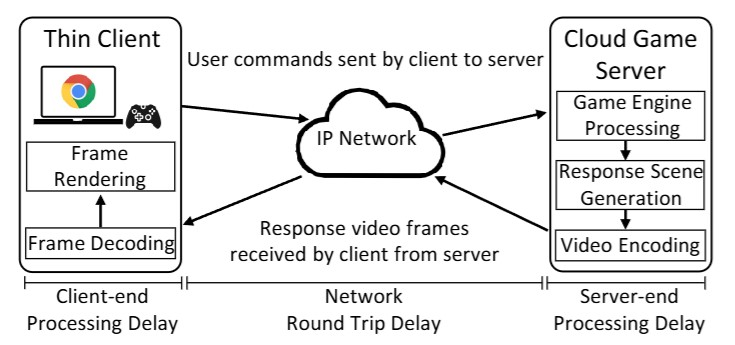
\includegraphics[width=.8\linewidth]{imgs/chapter_1/archi_cg.jpg}
    \caption{Cloud Gaming platform architecture \protect{\cite{Iqbal2021DissectingCG}}}
    \label{fig:chap_1:cg_architecture}
\end{figure*}

Commercial platforms, despite having the same broad architecture, have their specificities in terms of network protocols \cite{Iqbal2021DissectingCG, marchal2023analysis, Domenico2021ANA}. For instance, \ac{STD} and \ac{XC} rely on WebRTC: game commands are sent with \ac{DTLS} packets, video packets are encoded using H.264 and VP9 codecs and streamed using \ac{RTP} packets. \ac{GFN} uses \ac{UDP} to send user commands and also RTP for video streaming encoded using H.264 codecs. \ac{PSN} uses a custom implementation of \ac{UDP}.

Each platform specifies minimum bandwidth requirements for an optimal cloud gaming (CG) experience. However, they do not provide clear information on the maximum acceptable latency  despite its significant impact on user experience, as discussed later in this section. These recommendations are summarized in Tab. \ref{tab:cg_platforms}.
\begin{table*}[!ht]
\setlength\tabcolsep{1pt} 
    
\begin{tabular*}{\linewidth}{@{\extracolsep{\fill}} llll}
    \toprule
       \bf CG platforms & \bf Minimum Bandwidth & \bf Resolution & \bf Network protocols \\
    \addlinespace
    \cmidrule{1-4}
    \bf STD & 10/20/35Mbps & 720p/1080p/4K &  WebRTC \\ 
    \bf GFN & 15/25/45Mbps & 720p/1080p/4K & UDP \\
    \bf XC & 10Mbps & 1080p & WebRTC \\
    \bf PSN & 5/15/38Mbps & 720p/1080p/4K & UDP \\
    \bf Luna & 10/35Mbps & 1080p/4K & WebRTC \\
    \bottomrule

\end{tabular*}
\caption{Commercial CG platforms}
\label{tab:cg_platforms}
\end{table*}

\subsubsection{Factors impacting QoE in CG platforms}
Although \ac{CG} can remove the need of expensive computing hardware for gaming, streaming high-quality video gaming requires reliable and low-latency connections to avoid a bad user experience. \ac{QoE} is defined by \cite{le2013qualinet} as \textit{"the degree of delight or annoyance of the user of an application or service. It results from the fulfillment of his or her expectations with respect to the utility and/or enjoyment of the application or service in the light of the user’s personality and current state."}

According to ITU-T Rec G.1032 \cite{itut1032}, the factors of a CG that can influence the \ac{QoE} can be classified into three groups:
\begin{itemize}
    \item Human factors: These are linked to the characteristics of the user, such as gaming experience, vision and auditory capabilities, or intrinsic/extrinsic motivation.
    \item Context factors: These are related to the user’s environment, such as social context or physical surroundings (e.g., room characteristics or use in mobility versus at home).
    \item System factors: These refer to the properties that \textit{"determine the technically produced quality of an application or service"} \cite{itut1032}. This includes the game being played, the gaming setup (hardware and software), network transmission, and compression.
\end{itemize}

We focus here only on the network factors that impact the most the \ac{QoE} of cloud gaming applications.
\begin{itemize}
    \item \textbf{Delay:} In cloud gaming, delay—often referred to as button-to-pixel delay—represents the time elapsed between a user action and the corresponding visual feedback on the screen. This delay (as illustrated in Fig. \ref{fig:chap_1:cg_architecture}) can be broken down into:
    \begin{itemize}
        \item Network delay: This delay is intrinsic to network communication, as data must travel between the client and server. High delays disrupt responsiveness, rendering games less playable.
        \item Client-Side delay: Delays from this end are decreasing with advances in device performance and higher display refresh rates \cite{Kmrinen2017AMS}.
        \item Server processing delay: This delay varies by game and platform, depending on the server's capabilities and load \cite{Iqbal2021DissectingCG}.
    \end{itemize}

    The impact of delay on QoE has been been widely studied. Claypool et al. \cite{Claypool2014TheEO} demonstrated that high delays significantly degrade player performance on platforms like OnLive and GamingAnywhere, particularly for genres like racing and first-person shooters, which are more latency-sensitive than role-playing or strategy games. Peñaherrera-Pulla et al. \cite{PeaherreraPulla2021MeasuringKQ} identified latency as one of the key factors to ensure the responsiveness required for CG. Xu et al. \cite{Xu2022MeasurementOT} highlighted the impact of network congestion, showing that competing traffic (like \ac{TCP} traffics) can result in buffer bloat and thus increase delays and negatively impact QoE on platforms like \ac{STD}, \ac{GFN} and Luna.

     \item \textbf{Jitter:} Jitter is a measure of how inconsistent is the delay between packets. Jitter causes the video to be stuttered instead of being smooth. While video buffering can mitigate this in non-interactive applications like streaming, jitter poses a significant challenge in CG, where it directly impacts the \ac{QoE}.  Aumont et al. \cite{Aumont2021DissectingCG} demonstrated that jitter significantly impacts the gaming experience on CG platforms like \ac{STD} and \ac{GFN}. Oliveira et al. \cite{FlanaganEffectsOJ} confirmed these findings in their experiments on STD using four different games. They observed that high jitter magnitudes deteriorate the user experience on CG.

    \item \textbf{Bitrate:} The bitrate represents the number of bits transferred per unit of time. In CG, the bitrate (limited by the available bandwidth) determines the maximum frame rate and resolution achievable by the platforms. Some studies outlined that lowering the bitrate (with some bandwidth restrictions for example) leads to lower user experience. Suznjevic et al. \cite{suznjevic2016analysis} demonstrated in a study on GFN that reducing the bandwidth results in lower graphics quality (characterized by decreased resolution and frame rates) and thus resulting in lowers QoE scores.
    In a study analyzing the behavior of CG platforms under different network conditions, Marchal et al. \cite{marchal2023analysis} found that when the available bandwidth decreases, CG platforms adapt by reducing the bitrate. This typically results in a drop in frame rate and resolution (due to a reduction of the quantization factor that is responsible for video compression). While CG platforms do not adapt the same way to this network disturbance, all experience resolution degradation and some become unplayable when the bandwidth falls below the platform bandwidth requirements. Iqbal et al. \cite{Iqbal2021DissectingCG} observed that under constrained bandwidth conditions, CG platform cannot consistently provide 1080p/60 fps streaming.


    \item \textbf{Packet loss:} occurs when one or more packets traveling a network fail to reach their destination due to network congestion, radio frequency interferences or weak radio signals. Packet loss in CG applications significantly impacts user experience as demonstrated by Jarschel et al. \cite{jarschel2013gaming} on their experiment with an emulated CG platform. They observed that even a 1\% packet loss can reduce the \ac{MOS} score from 5 (excellent) to 2 (poor). Chen et al. \cite{chen2013quality} observed, using early CG platfors like OnLive and StreamMyGame, that packet loss affects the frame rate and the graphic quality. Thieir study revealed that former CG platforms do not implement robust packet loss concealment mechanisms. Similarly, Marchal et al. \cite{marchal2023analysis} found that \ac{PSN} does not allow to launch game sessions when packet loss exceed 5\%. In contrast, it was shown in \cite{Aumont2021DissectingCG, marchal2023analysis} that modern CG platforms like STD, GFN, XC are slightly impacted by packet loss as they used resilient error correction mechanisms including \ac{FEC} and high redundancy.
\end{itemize}


% Wang et al. \cite{Wang2012CloudMG} identified the gaming visual experience and the gaming response experience as the impairment factors affecting mobile \ac{CG}. Gaming visual experience depends on the video smoothness and the image quality which are linked to the bandwidth, packet loss and the compression process from the server while gaming response depends on the end-to-end delay. 



\subsection{Cloud VR}
\ac{VR} is a computer-generated experience where users can interact and feel immersed in a virtual environment. Traditional VR applications require high-end computers for the demanding graphics and processing for 3D immersive experiences, as most VR headsets cannot handle all the heavy computations and processing. As a result, the headsets are either tethered to the computer or wireless linked via technologies like AirLink to stream content.

Cloud \ac{VR} consists in offloading all the heavy computational tasks to cloud servers enabling real-time streaming of rendered VR content to lightweight and less expensive VR headsets. This approach reduces the need for powerful and costly computers, making VR more accessible and affordable. By removing the need on tethered setups, Cloud VR offers more mobility and flexibility enabling diverse use-cases of VR experiences. Cloud VR could also support scalability and fosters collaboration, opening opportunities for enterprises and institutions to develop innovative VR services.

According to \cite{huawei}, Cloud VR applications can be classified into two categories:
\begin{itemize}
    \item Weak-interaction VR that implies no interaction with the virtual environment. The users are passive and the contents are pre-determined. This includes 360 degree panoramic video, VR streaming or VR live broadcast.
    \item Strong-interaction VR includes VR services where user can interact in real-time with virtual environments through interactive devices for greater immersion. In these applications, the virtual environment depends on the inputs of the user unlike weak-interaction. This includes VR gaming, VR social networking (metaverses) and so on.
\end{itemize}
This thesis focuses only on strong interaction VR and Cloud VR will be used to refer to strong-interaction VR unless otherwise stated. 

\subsubsection{Factors impacting QoE in Cloud VR platforms}

As for CG, ITU-T Rec G.1035 \cite{itut1035} classified the factors that can influence the QoE in cloud VR into human, context and system factors.
The network factors impacting the Cloud VR experience are categorized based on the experience evaluation factors of Cloud VR, which according to \cite{huawei} are: \textbf{i) the sense of reality} which are determined by the quality of audio and video to allow the users to feel immersed and are directly impacted by the bandwidth; \textbf{ii) the sense of interaction} which are impacted by the latency and \textbf{iii) the sense of pleasure} that depends on the smoothness and can be impacted by the bandwidth, the latency and the packet loss.
Thus, as for CG, the most influencing network factors on QoE for Cloud VR are:
\begin{itemize}
    \item \textbf{Delay:} In VR, the delay, often referred as \textit{motion-to-photon} (MTP) delay, is the time elapsed between a user movement and the resulting change in the headset's field of view after rendering. In Cloud VR, the network latency adds to MTP delay because the VR content is streamed from the cloud. The impact of delay in Cloud VR were discussed in the literature. Song et al. \cite{song2022impact} demonstrated that increased latency results in black edge artifacts (that corresponds to black area in the viewport boundary when users turn their heads) affecting QoE. Their study highlighted the sensitivity of users to both the duration and size of these artifacts. Lee et al. \cite{lee2024adaptive} found that higher delays or lower frame rates contribute to cybersickness, further degrading the VR experience. Warsinke et al. \cite{warsinke2024vr} observed that even moderate additional delays (e.g., 40 ms) significantly affect VR session quality, with impacts varying by game genre.
    
    \item \textbf{Bandwidth:} Cloud VR applications are highly bandwidth-intensive due to higher resolutions, higher frame rates, coding technology used, extra-perspective rendering and transmission required to reduce the impact of black edge events. Bandwidth constraints can lead to reduce graphics quality and frame rates, affecting the user experience. \cite{huawei} reported that a minimum bandwidth of 80 Mbps is required for a fair-experience. Li et al. \cite{li2020performance} showed that insufficient bandwidth may causes congestion, reducing frame rates and compromising QoE. Their subjective studies confirmed that users notice and react negatively to these degradations. Lee et al. \cite{lee2024adaptive} identified a direct correlation between increased bitrate and better visual quality, using the MOS score of their QoE model.  

    \item \textbf{Packet loss:} It is recommended to use UDP for Cloud VR but since there is no retransmissions in UDP, packet loss can cause issues like visual quality degradations or black edge events. Li et al. \cite{li2020performance} confirmed with objective and subjective studies that packet loss disrupts frame rates and graphics, and affects user experience. Rossi et al. \cite{rossi2024subjective} observed in a subjective study, that packet loss rates as low as 12\% adversely affect throughput and frame rate, reducing the MOS. Warsinke et al. \cite{warsinke2024vr} highlighted that even minimal packet loss (0.3\%) significantly impacts VR gaming session quality.  



\end{itemize}

% These findings collectively emphasize that delay, bandwidth, and packet loss are critical determinants of QoE in Cloud VR. Addressing these factors is essential for enhancing the user experience and mitigating performance issues in Cloud VR applications.  

% On experiments on a cloud VR gaming platform (ALVR), Li et al. \cite{li2020performance} shown in objective studies that frame rate is impacted by insufficient bandwidth and packet loss. Latency is also impacted by these parameters as lower bandwidth lead to congestion. They also conduct subjective studies and shown that gaming experience are impacted by delay, bandwidth and packet loss.


% Song et al. \cite{song2022impact} prove the relationship between latency in cloud VR and black edge artifacts (that corresponds to black area in the viewport boundary when users turn their heads). They shown in subjective studies that the QoE are impacted by the duration and also the area of a black edge event as users easily noticed black edge events.


% Rossi et al. \cite{rossi2024subjective} showed on subjective QoE tests using a commercial Cloud VR solution that round-trip time, jitter and packet loss impact the MOS score. The Cloud VR gaming throughput was impacted by jitter and packet loss rate of 12\% while the frame rate was affected by \ac{RTT}.


% Lee et al. \cite{lee2024adaptive} shown in a user studies that the MOS score increase as the bitrate increases leading to better visual quality. They also shown that the QoE depends on the game genres that may have different requirements and that cyersickness occured with higher delays or lower frame rates. They also proposed and validated a QoE model based on network parameters like bandwidth, delay and packet loss which prove that they are impacting factors for QoE.


% Warsinke et al. \cite{warsinke2024vr} design a user study and shown that packet loss (0.3\%) and additional delay (40ms) impact the overall VR gaming session quality but the results differs depenging on the game genre.

% reinsérer dans les bullet points.

% \takeaway{Low-latency applications like CG and Cloud VR demand minimal delay and high network reliability to deliver interactive and immersive experiences. Their performance is influenced by factors such as latency, jitter, bitrate, and packet loss as highlighted by many studies in the literature.}

% \takeaway{\ac{LL} applications like cloud gaming, Cloud VR, video conferencing, and remote medical surgery share a need for minimal end-to-end delay, but their bandwidth and latency requirements differ. CG and Cloud VR, the focus of this thesis, demand high network reliability to deliver interactive and immersive experiences. These applications involve complex architectures and protocols, with network factors like delay, jitter, bitrate, and packet loss significantly impacting user experience as highlighted by many studies in the literature.}

% améliorer le lien

% \usage{This thesis focuses on CG and CloudVR as \ac{LL} applications. Data collection (Chapter \ref{chap:measurements}) was performed using commercial CG platforms and experimental versions of CloudVR systems. These datasets serve as the foundation for developing anomaly detection (Chapters \ref{chap:ml_evaluation}, \ref{chap:cats}) and root-cause diagnosis techniques (Chapter \ref{chap:diagnosis}).}


% \usage{This thesis focuses on anomaly detection and root-cause diagnosis for the performance of low-latency (LL) applications, with a specific emphasis on CG and Cloud VR. These applications were chosen due to their growing business relevance for Orange and their sensitivity to network performance issues. In Chapter \ref{chap:measurements}, we conduct data collection using commercial CG platforms and experimental Cloud VR systems under time-varying network conditions. These conditions are designed to replicate real-world scenarios prone to the network factors which can cause performance anomalies in LL applications. The resulting datasets provide the foundation for evaluating anomaly detection techniques in Chapters \ref{chap:ml_evaluation} and \ref{chap:cats}. Furthermore, they are used to evaluate our proposed solution for root-cause diagnosis of LL application performance issues, detailed in Chapter \ref{chap:diagnosis}.}

\section{Time varying capacity networks}
\subsection{Cellular Networks}


\begin{figure*}[!ht]
    \centering
    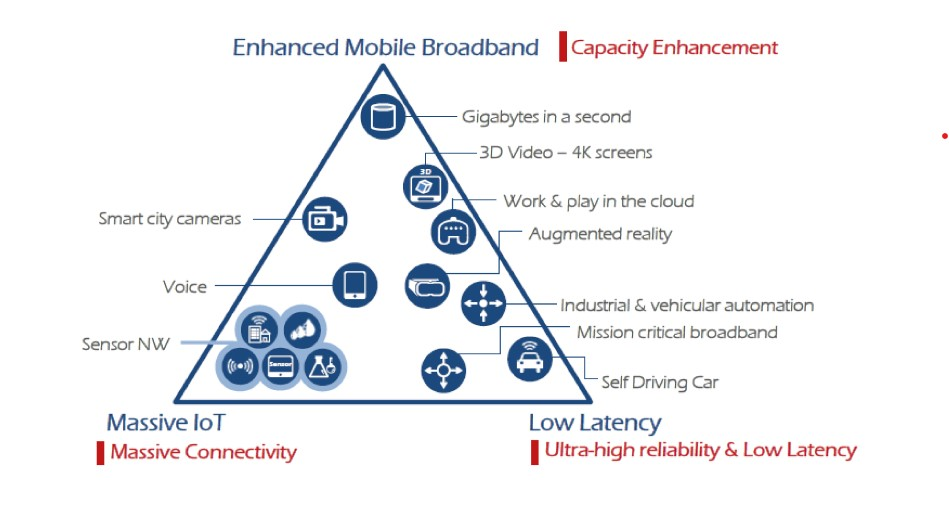
\includegraphics[width=.8\linewidth]{imgs/chapter_1/5g_app.jpg}
    \caption{ITU-T 5G requirements \protect{\cite{IMT_itut_2020}}}
    \label{fig:chap_1:5g_requirement}
\end{figure*}


Since the 1980s and the announcement of the 1st generation (1G) with a data rate of up to 2.4 kbps, each decade has seen the introduction of a new mobile cellular generation. The second generation (2G), launched in the 1990s, brought significant advancements over 1G, including services like \ac{SMS} text messaging. 2G supported communication with data rates of up to 144 kbps. 

The 3rd generation (3G), introduced in the 2000s, offered data rates ranging from 384 kbps to 42 Mbps (with its latest enhancements). 3G enabled new capabilities, such as convenient web browsing, and became the first cellular network widely adopted for diverse applications, including medical devices and fire alarms.

The 4th generation (4G), launched in the 2010s, was expanded by the \ac{ITU} to include the latest evolutions of 3G, such as \ac{LTE}, \ac{WiMAX}, and \ac{HSPA+}. It achieved speeds of up to 150 Mbps and featured reduced latency, improving the user experience for applications like video streaming, video conferencing, and gaming services.

The 5th generation (5G) began deployment in 2019, following its definition by \ac{3GPP} Release 15, which introduced \ac{5G NR} % add reference. 
Compared to LTE, 5G is expected to deliver up to 20 times the theoretical bandwidth of LTE (1 Gbps) and ultra-low latency down to 1 ms \cite{IMT_itut_2020}. 

5G is designed to address three key application scenarios, as illustrated in \ref{fig:chap_1:5g_requirement}:
\begin{itemize}
    \item \ac{eMBB}, providing faster connections with higher bandwidth (up to 20 Gbps) and moderate latency, suitable for applications like AR/VR, cloud gaming, and 360-degree video streaming.
    \item \ac{URLLC}, supporting ultra-low latency (down to 1 ms) and high reliability (99.999\%) for mission-critical applications, such as Industry 4.0 processes and remote healthcare.
    \item \ac{mMTC}, enabling connectivity for a large number of \ac{IoT} devices (up to $10^6$ per square kilometer), albeit with trade-offs in throughput and latency.
\end{itemize}


\subsubsection{Architecture of 4G/5G networks}



\begin{figure*}[!ht]
    \centering
    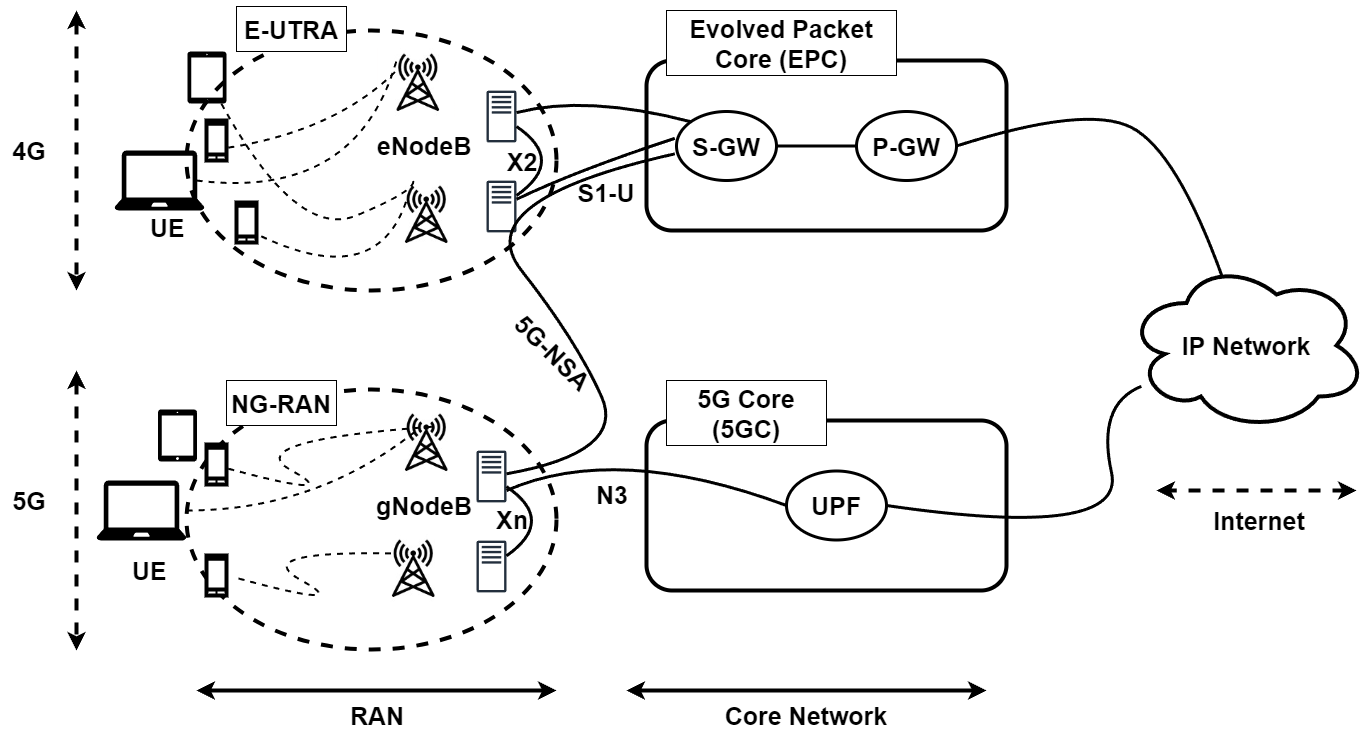
\includegraphics[width=.8\linewidth]{imgs/chapter_1/cellular_network.png}
    \caption{Cellular networks architecture (focus on user-plane)}
    \label{fig:chap_1:cellular_network}
\end{figure*}

The architecture of a cellular network, depicted in Fig. \ref{fig:chap_1:cellular_network}, consists of three main parts: the \ac{UE}, \ac{RAN}, and the core network. The core network connects the RAN to external networks (e.g., \ac{IP} networks), while the RAN provides connectivity between UEs and the mobile core network. In 4G (resp. 5G), the RAN is referred to as \ac{E-UTRA} (resp. \ac{NG-RAN}), and the mobile core network is known as \ac{EPC} (resp. \ac{5GC}).

The primary component of the RAN is the \ac{BS}, referred to as \ac{eNB} in 4G and \ac{gNB} in 5G. UEs connect to the BS through the radio air interface, and the BSs are linked to the core network. In 4G, BSs are interconnected via the X2 interface (resp. Xn interface in 5G) to facilitate handovers between neighboring cells. They are connected to the core network via the S1 interface (resp. N3 interface in 5G). 

The 4G \ac{EPC} comprises several key components. The \ac{MME} handles user authentication, mobility management, and signaling. The \ac{S-GW} manages the user data plane, while the \ac{P-GW} serves as a gateway connecting the network to external IP networks. 

In contrast, the 5GC is designed to be more flexible and cloud-aligned using a \ac{SBA}, where network functions are decoupled and deployed as microservices using \ac{NFV}. Key components of the 5GC include the Access and Mobility Management Function (AMF), which replaces the MME in 4G and handles connectivity and mobility management; the User Plane Function (UPF), which assumes the data routing roles of the SGW and PGW; and the Session Management Function (SMF), which manages session establishment and \ac{QoS}. 

The 5G architecture introduces advanced concepts such as network slicing, \ac{MEC}, and the use of a wider range of frequency bands (e.g., mmWave) to achieve higher throughputs and lower latency, supporting next-generation applications like low-latency services. 

Early 5G deployments used the \ac{NSA} architecture, which leverages \ac{5G NR} in the RAN to enhance data speeds while relying on the 4G EPC for control plane functions. This approach enabled faster initial 5G rollouts by requiring fewer infrastructure changes. However, \ac{NSA} cannot deliver the full potential of 5G, such as ultra-low latency and network slicing. Full \ac{SA} deployments, which use 5G NR along with the cloud-native 5G core, are expected to realize the complete range of capabilities promised by 5G networks.



\subsection{Wi-Fi networks}

Wi-Fi is a trademark of the Wi-Fi Alliance, commonly used to refer to wireless \ac{LAN}s based on IEEE 802.11 standards. Wi-Fi is used to connect devices such as laptops, smartphones, \ac{IoT} devices, and gaming consoles to the Internet via a wireless router. It enables short-range wireless communication in environments such as campuses, homes, and restaurants. Any device capable of connecting to a wireless network is referred to as a station and is equipped with a wireless network interface controller. Stations are categorized into two types: \ac{AP}s and clients.



\subsubsection{Architecture of Wi-Fi networks}

Wi-Fi networks are primarily deployed in infrastructure mode, where all communications pass through an AP. In this mode, a Wi-Fi network architecture comprises one or more APs, one or more client devices connected to the AP, and a distribution system (typically a wired Ethernet connection) that links the AP to the Internet. The AP broadcasts to the clients a \ac{SSID} to identify the network, using beacon packets. To access the Internet, a client sends an association request to the AP, which authenticates the client using security protocols such as \ac{WPA} (e.g., WPA2/WPA3). Once authenticated, the client is assigned an IP address by the \ac{DHCP} server on the AP, enabling Internet connectivity.

% Figure architecture Wi-Fi


\subsubsection{Evolution of WiFi standards with performance characteristics}

The first Wi-Fi standard, IEEE 802.11, was released in 1997. Operating at 2.4 GHz, it offered data rates of up to 2 Mbps. However, it faced limited adoption due to interoperability issues, insufficient throughput, and weak security. In 1999, IEEE 802.11b (Wi-Fi 1) improved upon this by achieving theoretical data rates of up to 11 Mbps at 2.4 GHz and a range of up to 300 meters in clear environments. Wi-Fi 1 gained popularity for basic Internet browsing and email but suffered from interference issues due to sharing the 2.4 GHz band with other wireless technologies like Bluetooth and microwave ovens.

IEEE 802.11a (Wi-Fi 2) was introduced alongside Wi-Fi 1, operating on the less-crowded 5 GHz band with data rates of up to 54 Mbps. However, its higher frequency required more expensive antennas to maintain range, and it was not interoperable with Wi-Fi 1. 

In 2003, IEEE 802.11g (Wi-Fi 3) combined the strengths of 802.11b and 802.11a by operating on the 2.4 GHz band while offering data rates of up to 54 Mbps. It was backward compatible with 802.11b, making it a popular choice for commercial use.

Released in 2009, IEEE 802.11n (Wi-Fi 4) brought significant improvements in speed and reliability. It introduced \ac{MIMO} technology, allowing multiple antennas to transmit and receive data simultaneously, achieving data rates of up to 600 Mbps. It also supported dual-band support (2.4 and 5 GHz), offering better range and reduced interference.

Built on the advancements of 802.11n, IEEE 802.11ac (Wi-Fi 5), launched in 2013, further enhanced Wi-Fi performance by operating exclusively on the 5 GHz band, offering gigabit speeds of up to 3.5 Gbps. Features such as advanced MIMO configurations, beamforming, and wider channel bandwidths made it ideal for applications like \ac{HD} and 4K video streaming, gaming, and video conferencing. It remained backward compatible with previous standards.

IEEE 802.11ax (Wi-Fi 6 and later Wi-Fi 6E) improved performance, scalability, and energy efficiency with \ac{OFDMA} technology. Wi-Fi 6 operates on the 2.4 GHz and 5 GHz bands, while Wi-Fi 6E adds the 6 GHz band, providing additional spectrum and reducing congestion. With speeds of up to 9.6 Gbps, this standard is ideal for environments with many connected devices, such as smart homes and IoT ecosystems.

The upcoming IEEE 802.11be (Wi-Fi 7) standard aims to further enhance performance, delivering data rates of up to 46 Gbps and ultra-low latency. It is designed to support advanced applications like AR/VR, 8K streaming, and immersive experiences.

The evolution of Wi-Fi standards is summarized in Tab. \ref{tab:wifi_standard}.

\begin{table*}[!h]
\setlength\tabcolsep{1pt} 
    
\begin{tabular*}{\linewidth}{@{\extracolsep{\fill}} lccccc}
    \toprule
       & \bf IEEE 802.11 & \bf Release & \bf Frequency & \bf Channel & \bf Max \\
       & \bf protocol & \bf Date & \bf Band (GHz) & \bf Bandwidth (MHz) & \bf Throughput \\
    \addlinespace
    \cmidrule{1-6}
            & 802.11 & 1997 & 2.4 & 22 & 2 Mbps \\
    Wi-Fi 1 & 802.11b & 1999 & 2.4 & 22 & 11 Mbps \\
    Wi-Fi 2 & 802.11a & 1999 & 5 & 20 & 54 Mbps \\
    Wi-Fi 3 & 802.11g & 2003 & 2.4 & 20 & 54 Mbps \\
    Wi-Fi 4 & 802.11n & 2009 & 2.4 & 20/40 & 600 Mbps \\
    Wi-Fi 5 & 802.11ac & 2013 & 5 & 20/40/80/160 & 3.5 Gbps \\
    Wi-Fi 6 & 802.11ax & 2019 & 2.4/5 & 20/40/80/160 & 9.6 Gbps\\
    Wi-Fi 6E & 802.11ax & 2020 & 2.5/5/6 & 20/40/80/160 & 9.6 Gbps \\
    Wi-Fi 7 & 802.11be & 2024 (expected) & 2.5/5/6 & 20/40/80/160/320 & 46.1 Gbps \\
    \bottomrule

\end{tabular*}
\caption{Evolution of Wi-Fi standards}
\label{tab:wifi_standard}
\end{table*}
% https://www.wevolver.com/article/the-evolution-of-wi-fi-networks-from-ieee-80211-to-wi-fi-6e


\subsection{LL applications performance under time-varying capacity network}
Low-latency applications such as CG and Cloud VR require high-performance networks to ensure acceptable \ac{QoS}/\ac{QoE}. However, their performance is significantly affected by time-varying network capacity. This section synthesizes insights from the literature on how CG and Cloud VR perform under such network conditions.

\subsubsection{Performance on cellular networks}
Kamarainen et al. \cite{Kmrinen2017AMS} found that LTE networks deliver stable network delays under strong signal conditions (RSRP between -50 and -70 dBm). However, noticeable delay fluctuations occur with weaker signals (-100 dBm or more), and latency can increase 2-4 times under poor conditions.
Domenico et al. \cite{Domenico2021ANA} examined cloud gaming performance on 3G and 4G networks using \ac{STD} as a benchmark. They observed that STD struggles to stream on 3G, even under optimal conditions. In contrast, 4G networks can support resolutions up to 4K with excellent signal quality, although poor 4G conditions lead to abrupt streaming interruptions.
Tan et al. \cite{tan2018supporting} highlighted LTE’s signaling inefficiencies, such as inter-protocol incoordinations and single-protocol overhead, which contribute to network latency often exceeding the 25 ms threshold required for acceptable VR performance.
Bhuyan et al. \cite{bhuyan2022end} demonstrated that 5G networks can handle 4K CG streams with high bitrates (up to 50 Mbps). However, frame drops occur due to larger game frame sizes and buffering-induced packet loss. These frame drops are significantly reduced when the bitrate is lowered to 30 Mbps. The study also revealed that 5G is 46\% more energy-intensive than Wi-Fi, mainly due to its use of higher frequencies and the power demands of mmWave antennas.
Penaherrera et al. \cite{penaherrera2024cloud} validated that standalone 5G (5G SA) networks effectively support Cloud VR applications. However, combining 5G SA with WiFi 6 increases latency due to Wi-Fi's higher uplink latency in WiFi. In mobility scenarios, 5G outperforms WiFi by offering higher throughput and more stable latencies.


\subsubsection{Performance on WiFi networks}
Maiorano et al. \cite{maiorano2022local} demonstrated that the performance of Cloud VR applications, such as NVIDIA’s CloudXR, deteriorates as the distance between the headset and router increases. Low bandwidth reduces frame rates while signal attenuation increases delay.
Zhang et al. \cite{zhang2018wifi} revealed that Wi-Fi 5 struggles with Cloud VR due to high \ac{RTT} of up to 228 ms and jitter levels that exceed the recommended thresholds for real-time applications.
Jansen et al. \cite{jansen2023can} showed that signal attenuation on Wi-Fi networks causes bandwidth fluctuations, destabilizing throughput and affecting Cloud VR performance. The 5 GHz band offers higher bandwidth than the 2.4 GHz band but is more susceptible to signal attenuation.
Penaherrera et al. \cite{penaherrera2024cloud} demonstrated that Wi-Fi 6 provides superior latency performance for Cloud VR compared to 5G in stationary scenarios. However, its uplink performance remains a limiting factor.
Burbano et al. \cite{burbano2024impact} emphasized that even Wi-Fi 6 struggles to maintain stable Cloud VR sessions under high traffic congestion, particularly on the 2.4 GHz band.



\subsubsection{Key Observations Across Networks}

Studies such as \cite{Domenico2021ANA, bhuyan2022end} emphasize the importance of adequate bandwidth in ensuring the performance of low-latency applications. While 5G offers superior capacity, Wi-Fi remains limited by its inherent constraints, especially in older protocols. Cellular networks, particularly 5G, excel in providing low-latency connections. However, inefficiencies in LTE protocols and signal attenuation in Wi-Fi can significantly degrade performance. Additionally, \cite{bhuyan2022end} highlights that Wi-Fi is more energy-efficient than 5G for CG and Cloud VR, making it more suitable for stationary use cases. Finally, the performance of both 4G and Wi-Fi is heavily dependent on signal quality, with poor conditions exacerbating latency, jitter, and packet loss.



%\takeaway{Cellular networks offer varying levels of bandwidth and latency, with 5G enabling ultra-low latency for mission-critical applications. Wi-Fi protocols have evolved to support higher data rates. However, user experience of LL applications under these networks are often challenging as  time-varying capacity networks may present bandwidth unavailability and latency instability due to multiple causes.} % change suboptimal


% \takeaway{Cellular networks have evolved from 1G to 5G, with 5G offering ultra-low latency, enhanced bandwidth, and novel concepts like network slicing and edge computing. Similarly, Wi-Fi standards have progressed from IEEE 802.11 to Wi-Fi 7, delivering higher throughput and reduced latency. Despite these advancements, both network types face multiple challenges resulting in bandwidth unavailability and latency instability, which impact performance of \ac{LL} applications.}



% \usage{This thesis focuses on evaluating \ac{LL} applications under challenging network environments, specifically 4G and Wi-Fi. The experimental testbeds for data collection (Chapter \ref{chap:measurements}) were designed to reproduce realistic scenarios within these networks, thus capturing the performance impacts and challenges faced by LL applications in such environments.}
 








    
    % Jansen et al. Can My WiFi Handle the Metaverse? A Performance Evaluation Of Meta’s Flagship Virtual Reality Hardware
    
    % Casasnovas et al. Experimental evaluation of interactive Edge/Cloud Virtual Reality gaming over Wi-Fi using unity render streaming

    % Penaherrera et al. \cite{penaherrera2022kqi} KQI Assessment of VR Services: A Case Study on 360-Video Over 4G and 5G





    % Michaelides et al. Is Wi-Fi 6 Ready for Virtual Reality Mayhem? A Case Study Using One AP and Three HMDs



\section{Machine Learning paradigms}
\ac{ML} is a branch of \ac{AI} that uses algorithms capable of learning from data and generalizing to unseen data to perform specific tasks. Tom Mitchell (1997) proposed an engineering-oriented definition of ML: "\textit{A computer program is said to learn from experience E with respect to some task T and some performance measure P, if its performance on T, as measured by P, improves with experience E}."

\ac{DL} is a subset of ML based on multi-layered neural networks (hence the term \textit{deep}) to model complex patterns in large datasets. DL has demonstrated remarkable success in various fields, such as computer vision and natural language processing, due to its ability to automatically extract relevant features from raw data. 
% Neural networks were inspired from the human brain

The simplest neural network architecture, the perceptron, was invented by Frank Rosenblatt in 1957. It was sufficient for solving linearly separable tasks but limited in handling non-linear problems. Neural networks were subsequently improved to address increasingly complex tasks. Examples of key advancements include:
\begin{itemize}
    \item \textbf{\ac{MLP}} (1958): consists of multiple layers of neurons including at least one hidden layers, an input layer and an output layer. With backpropagation, MLPs was capable to solve non-linear problems.
    \item \textbf{\ac{CNN}}: are space-invariant neural networks that learns features using convolution kernels (or filters) sliding across input features. CNNs gained popularity for image processing tasks but can also be applied to signal processing.
    \item \textbf{\ac{RNN}}: designed for sequential data processing, such as time series or text, RNNs maintain a memory of previous inputs. They were enhanced with \ac{LSTM} and \ac{GRU} architectures to effectively capture long-term dependencies.
    \item \textbf{Autoencoders}: consist of an encoder that compresses input data into a latent space and a decoder that reconstructs the input from its latent representation. Autoencoders are primarily used in unsupervised learning for dimensionality reduction and later for representation learning and generative tasks with multiple variants.
    \item \textbf{\ac{GAN}} (2014): comprised of two networks with opposite goals- a generator and a discriminator- that contest in a zero-sum game resulting in a generator capable of generating highly realistic data.
    \item \textbf{Transformers} (2017): an architecture that has revolutionized many tasks including \ac{NLP}, \ac{CV}, and more, utilizing multi-head attention mechanisms to focus on different part of a sequence simultaneously. Transformers are at the core of architectures like \ac{ViT}, and \ac{LLM} achieving state-of-the-art results across various domains and benchmarks.
\end{itemize}


\subsection{Learning paradigms}


In ML, various learning paradigms are tailored to specific tasks and the availability of training data. Among these, only the paradigms relevant to this thesis are discussed, as depicted in Fig. \ref{fig:chap_1:ml_paradigms}.

\begin{figure*}[!ht]
    \centering
    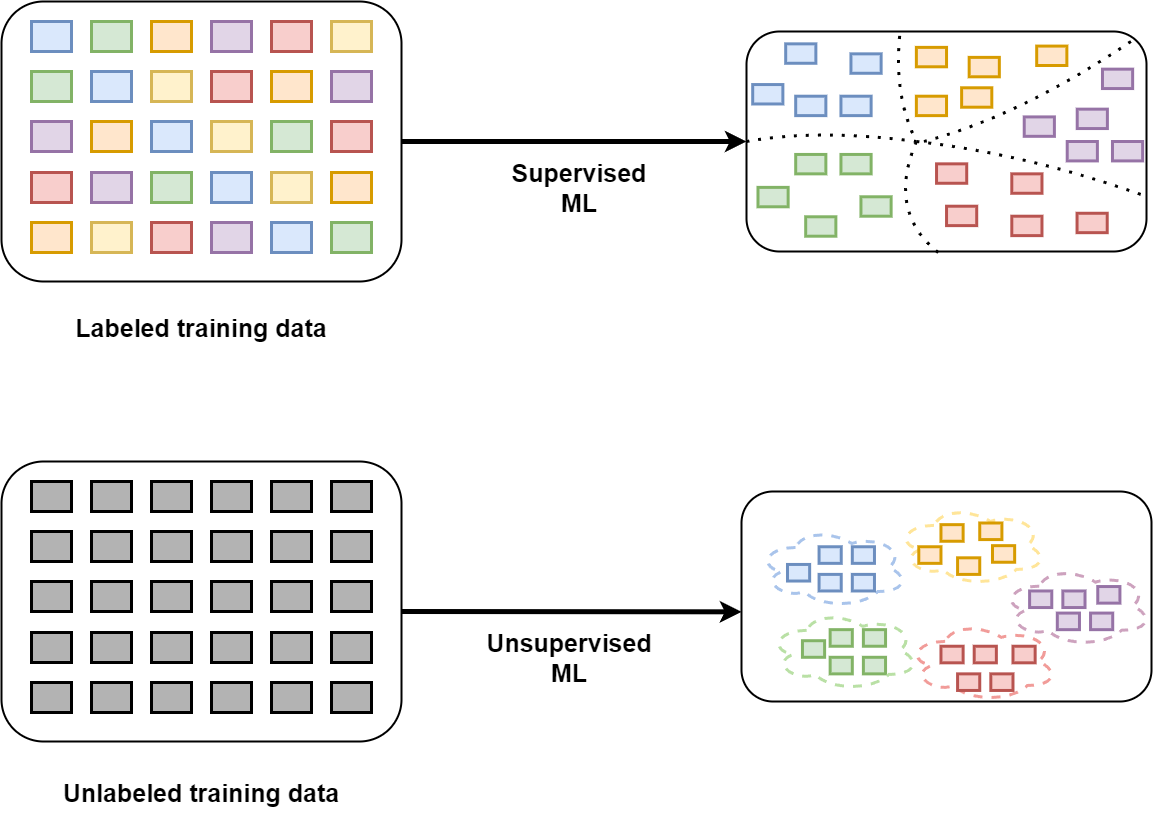
\includegraphics[width=.7\linewidth]{imgs/chapter_1/learning_paradigm.png}
    \caption{Machine learning paradigms}
    \label{fig:chap_1:ml_paradigms}
\end{figure*}

\subsubsection{Supervised learning}
\ac{SL} is the most fundamental and widely used learning paradigm. In SL, the training dataset $\mathcal{D}_{train} = \{(x_1, y_1), ..., (x_N,y_N)\}$ consists of a sufficient and representative amount of labeled samples (input-label pairs) that serve to learn a function $f_{\theta}$ approximating the true underlying relationship between $x_i$ and $y_i$.  
%that will determine the correct label for an unseen value $\tilde{x_i}$ and thus

The common SL tasks are classification tasks where we learn how to map the input $x_i$ to a discrete label (also category or class) and regression tasks where we map the input to a continuous value.

While effective for certain tasks, SL has notable limitations:
\begin{itemize}
    \item \textbf{Amount of labels}. SL requires a large amount of labeled data for training. However, the acquisition of these labels is often time-consuming and resource-intensive and may demand expert knowledge in domains such as networking or healthcare.
    \item \textbf{Label quality}. If the labels are erroneous, (which is possible since annotation process is done by humans), it can negatively impact the model performance.
    \item \textbf{Generalizability and overfitting}. SL models may require complex architectures to capture the underlying patterns in the training data. This complexity can lead to overfitting, causing poor performance on unseen data or data with different distribution.
    \item \textbf{Scalability}. The performance of SL improves with larger datasets. However, increasing the dataset size requires substantial computational resources and higher annotation costs, which may become impractical.
\end{itemize}


\subsubsection{Unsupervised learning}

\ac{UL} is a learning paradigm in which, unlike \ac{SL}, the learning process is conducted on unlabeled data. The model uncovers hidden patterns or relationships in the data without explicit guidance. UL can involve tasks such as discriminative, dimensionality reduction, or generative tasks. Generative UL focus on modeling the data distribution by learning a parametric approximation $p_{\theta}$ of the true data distribution $p$ enabling the generation of data samples $x_i \in \mathcal{D}$. Dimensionality reduction involves representing high-dimensional datasets in low-dimensional feature spaces while preserving intrinsic dataset properties. It is useful for tasks like noise reduction, data visualization, and reducing computational time and memory usage, especially before applying ML algorithms that struggle with high-dimensional data. Discriminative UL identifies relationships or boundaries between samples based on their similarities and differences. This can be achieved through clustering, which organizes samples into groups (clusters) based on these relationships, or through representation learning. Representation learning aims to construct feature extractors that identify the most meaningful and insightful representations from input data, enhancing downstream tasks and generalization to unseen data.


\subsubsection{Self-supervised learning}

\begin{figure*}[!ht]
    \centering
    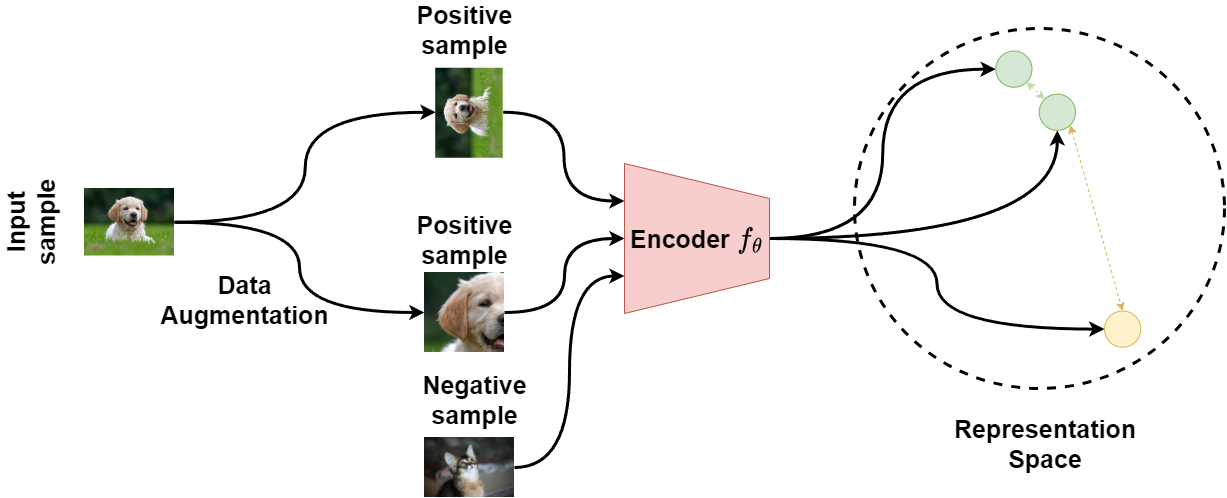
\includegraphics[width=.8\linewidth]{imgs/chapter_1/contrastive_learning.png}
    \caption{Contrastive learning}
    \label{fig:chap_1:contrastive_learning}
\end{figure*}

\ac{SSL}, a subset of UL, has gained immense popularity due to its remarkable performance across various tasks in \ac{NLP} and \ac{CV}. SSL leverages pseudo-labels derived from the inherent structure of unlabeled data to train models via pretext tasks. By solving these pretext tasks, the model generates self-supervision signals, enforcing it to learn task-agnostic features that capture essential patterns in the data (representation learning). Pretext tasks are designed based on the intended downstream tasks and typically include: i) \textbf{input completion} which consists in masking parts of the input and predicting the missing segments (e.g., predicting the next word in a sentence or reconstructing a portion of an image); ii) \textbf{transformation predictions} which consists in predicting transformations applied to the input (e.g., determining an image's rotation) or iii) \textbf{transformation invariance} which consists in learning invariant and meaningful features common across different representations of the same input after various transformations (e.g., using data augmentations).

Among SSL methods, \ac{CL} stands out as one of the most efficient and widely adopted frameworks. Its core idea, illustrated in Fig. \ref{fig:chap_1:contrastive_learning} involves training a feature extractor to cluster similar data (\textit{positive pairs}) in the feature space while pushing apart dissimilar data (\textit{negative pairs}). The key elements of CL include:
\begin{itemize}
    \item \textbf{Pair Selection:} Positive pairs and negative pairs are often generated using data augmentation. For example, in image classification, positive pairs can be created by applying different random crops or rotations to the same image, while negative pairs are generated by randomly selecting different images from the dataset.
    \item \textbf{Contrastive loss functions:} These include contrastive loss \cite{chopra2005learning}, triplet loss \cite{schroff2015facenet}, and InfoNCE loss \cite{oord2018representation}. The most commonly used is the \ac{NT-Xent} loss \cite{chen2020simple}. The most commonly used is \ac{NT-Xent} loss \cite{chen2020simple} which is defined as follows. 
    
    Given a mini-batch $\mathcal{B} = \{x_1, x_1^+, x_2, x_2^+, ..., x_N, x_N^+\}$ where $x_i^+$ is an augmented version of $x_i$, an encoder function $f_{\theta}$, NT-Xent loss will maximize the similarity between a representation of a sample $z_i = f_{\theta}(x_i)$ with its positive $z_i^+$ while minimizing its similarity with the $2N -2$ negatives $(z_j)_{\forall j \neq i \in \|1; N\|}$. The similarity is often measured with cosine similarity measure and the NT-Xent loss $\mathcal{L}_{NTXent}$ can be expressed as follows:

    \begin{equation}\label{eq:ntxent}
        \mathcal{L}_{NTXent} = - \frac{1}{2N} log \frac{exp(sim(z_i, z_i^+)/\tau)}{\sum_{k=1}^{2N} \mathbb{1}_{[k \neg i]} exp(sim(z_i, z_k)/\tau)}
    \end{equation}

    with $\tau$ a temperature hyperparameter that controls the relative importance of distance between pairs of points.
\end{itemize}

% Contrastive learning in general

% Contrastive learning on time series

\subsection{Training DL model}
Implementing a DL model involves a series of steps aimed at determining and optimizing the model's parameters by minimizing a loss function, ultimately achieving maximum performance on a given task. The process, summarized in Fig. \ref{fig:chap_1:dl_pipeline} is described as follows:
% Add figure of the pipeline


\begin{figure*}[!ht]
    \centering
    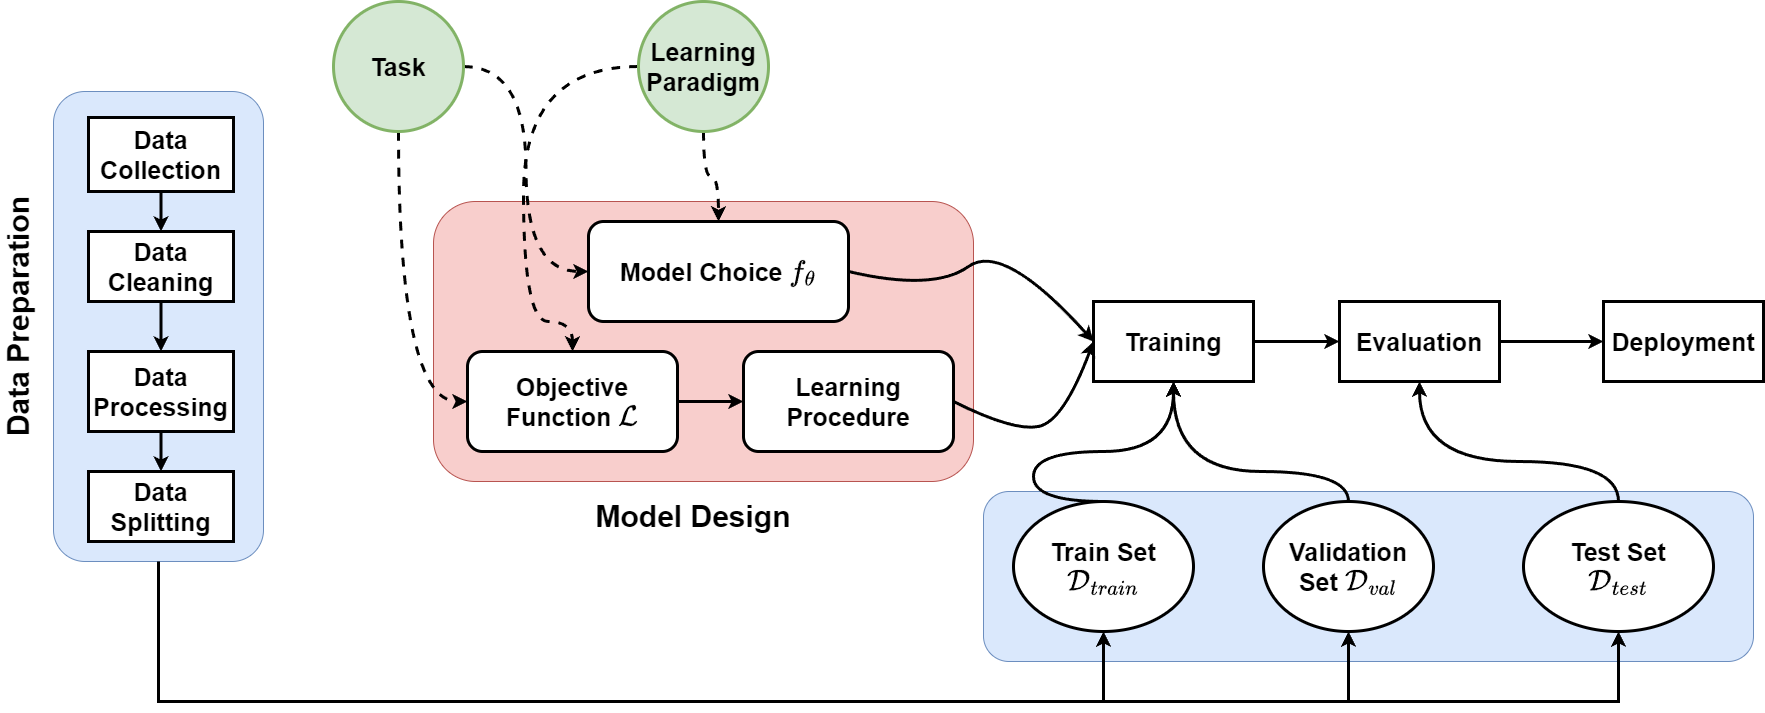
\includegraphics[width=.9\linewidth]{imgs/chapter_1/dl_pipeline.png}
    \caption{Deep learning implementation pipeline}
    \label{fig:chap_1:dl_pipeline}
\end{figure*}

\subsubsection{Dataset preparation}
The performance of a deep learning model is closely linked to the quality of the dataset. Preparing the dataset involves the following steps:

\begin{itemize}
    \item \textbf{Data collection :} Gather datasets that represent the problem domain. For this thesis, the focus is on time-series datasets for cloud gaming (CG) anomaly detection and virtual reality (VR) root-cause diagnosis.
    \item \textbf{Data cleaning :} Identify and remove missing, inconsistent or erroneous values in the dataset to ensure high-quality data.
    \item \textbf{Data processing :} Prepare data for model input through the following:
        \begin{itemize}
            \item Standardization/Normalization: Scale numerical features to a range (e.g., [0, 1]) or normalize them to have zero mean and unit variance.
            \item Categorical feature encoding: Apply one-hot or ordinal encoding for categorical features.
            \item Feature selection: Remove irrelevant or redundant features to improve learning efficiency. 
        \end{itemize}
    \item  \textbf{Data splitting :} the data should be split in three (03) sets. The training set used for the training of the model, the validation set to evaluate the model's performance during the training and the test set to assess the model's final performance and its generalizability.
\end{itemize}


\subsubsection{Design stage}
This stage involves selecting or defining the neural architecture ($f_{\theta}$) appropriate for the task and data type. To train the model, it is necessary to specify a loss function ($\mathcal{L}$), which quantifies the discrepancy between the model's outputs and the desired outputs (e.g., true labels in supervised learning). Common choices for the loss function include cross-entropy for classification tasks in supervised learning and reconstruction errors for autoencoders in unsupervised learning. The subsequent step is to choose an optimization technique to enhance the model's convergence speed and performance. The most widely used optimizers are \ac{SGD} and \ac{Adam}.


\subsubsection{Training stage}
The training stage is crucial as it aims to find the parameters that optimize task performance while ensuring generalizability. This involved solving an optimization problem that iteratively updates the model's parameters using only first-order derivatives. However, due to the large datasets typically used, calculating gradients across the entire dataset is impractical. Therefore, training is conducted using mini-batches (i.e., small subsets of training instances) and iterated over the entire dataset. The training process includes the following steps:
\begin{itemize}
    \item Sample a mini-batch $\mathcal{B} = {x_1, \ldots, x_{N_B}}$ from the training dataset.
    \item Perform a forward pass through the neural network to compute the outputs $f_{\theta}(x_i)$ for each sample ($x_i$) in the mini-batch.
    \item Calculate the average loss over all instances in the mini-batch: $\frac{1}{N_B} \sum_{i}^{N_B} \mathcal{L}(y_i, f_{\theta}(x_i))$.
    \item Compute gradients for model parameters with respect to the loss using backpropagation.
    \item Update the model parameters using an optimizer (e.g., SGD, Adam).
\end{itemize}


This setup is standard for supervised learning. For unsupervised or contrastive learning tasks, additional steps may be required. Hyperparameter tuning (e.g., learning rate, batch size, and number of epochs) is often necessary to enhance performance, alongside regularization techniques to mitigate overfitting.

\subsubsection{Evaluation stage and deployment}
After training, the model's performance is assessed on a test set using task-specific evaluation metrics. If the model demonstrates sufficient generalizability, it can be deployed in production environments. Post-deployment, it is essential to monitor the model's performance on new data to ensure continued effectiveness, and retraining may be necessary if performance declines.


%\takeaway{Deep learning (DL) leverages neural networks to design inference functions that solve tasks through various learning paradigms. Constructing a DL pipeline involves several key steps, which must be tailored to the specific task at hand. The goal is to create a model that is as generalizable as possible, ensuring its effectiveness when deployed in real-world applications.} % reformuler lien choix UL


% \takeaway{\ac{ML} and \ac{DL} have become essential for addressing complex problems across various domains. DL leverages neural networks, which excel in capturing intricate patterns, to design inference functions that solve tasks through various learning paradigms, including supervised, unsupervised, and self-supervised learning. Building a DL solution involves several key steps such as data preparation, model design, training, evaluation, and deployment, ensuring the performance and generalizability required for deployment in real-world scenarios.}


% \usage{In this thesis, we will follow this same DL implementation procedure, when designing ML solutions either for anomaly detection (Chapters \ref{chap:ml_evaluation}, , \ref{chap:cats}) or root-cause diagnosis (Chapter \ref{chap:diagnosis}).} % reformuler lien choix UL

\section{Anomaly Detection on time series}

% Intro sentence
Large amounts of multivariate time series data are generated across various domains, such as monitoring systems, finance, healthcare, networking, and security. The presence of anomalies in these time series can indicate malicious activity, fraud, cyber threats, system malfunctions, or diseases in healthcare. Consequently, detecting anomalies in time series data is becoming increasingly critical and has become a prominent area of research. Before delving into existing anomaly detection methods, we define the problem and introduce some key definitions.


% Define what a time series
\begin{definition}[Time series]
    A time series is a sequence of data points chronologically collected and equally-time spaced. Time series can be univariate or multivariate.
\end{definition}
A multivariate time series is formally defined as $X = \{ x_1, x_2, ..., x_T\}$ where $x_t \in \mathbb{R}^m$ denotes a $m$-dimensional vector corresponding to the observations of the $m$-features at a specific time $t$. A univariate time series is the special case when $m=1$. In this thesis, we focus on multivariate time series.

% Challenge of time series


% Define what is an anomaly
\begin{definition}[Anomaly]
    "\textit{An anomaly is an observation that deviates considerably from some concept of normality.}" \cite{ruff2021unifying}.
\end{definition}
Chandola et al. \cite{chandola2009anomaly} proposed a taxonomy of anomalies based on their nature:
\begin{itemize}
    \item \textbf{Point anomalies.} An individual data point that significantly differs from the rest of the data. This is the simplest type of anomaly. For instance, in fraud detection, an unusually high transaction amount compared to typical spending patterns is a point anomaly.
    \item \textbf{Contextual anomalies.}  A data point, anomalous in one context but normal in another. For instance, a temperature of 30°C is normal in the summer but anomalous in winter.
    \item \textbf{Collective anomalies.} A set of data points that, when considered together, represent an anomaly. Individually, each point may not be anomalous, but as a group, they indicate abnormal behavior. For instance, in a network monitoring system that typically processes 200–500 packets per minute, a steady rate of 450 packets per minute over 10 minutes might signal a collective anomaly.
\end{itemize}


\ac{AD} encompasses techniques for identifying data that deviate from normal patterns. While the terms \textit{anomaly}, \textit{outlier}, and \textit{novelty detection} are often used interchangeably, they have distinct meanings depending on the context. According to Ruff et al. \cite{ruff2021unifying}, given the distribution $\mathbb{P}^+$, of normal samples, an anomaly is an observation from a distribution different from $\mathbb{P}^+$. An outlier is a rare or a low-probability instance drawn from $\mathbb{P}^+$ while a novelty is an instance drawn from a new region of a non-stationary distribution of $\mathbb{P}^+$. For example, if $\mathbb{P}^+$ denotes the distribution of dogs, a cat would be an anomaly, a rare breed of dog an outlier and a newly discovered dog breed would be a novelty.  Despite their differences, these concepts share common detection methods, and this thesis collectively refers to them under the term anomaly detection.

For a multivariate time-series dataset $X = \{ x_1, x_2, ..., x_T\}$ with $x_t \in \mathbb{R}^m$, AD involves learning a model $f_{\theta}$ that assigns, for each unseen observation $\tilde{x_t}$, a label $y_t \in \{0, 1\}$ indicating whether the new observation is anomalous ($y_t = 1$) or not ($y_t = 0$). Depending on the learning setting, time series AD algorithms can be supervised, semi-supervised or unsupervised. This thesis focuses on reviewing unsupervised and self-supervised AD algorithms as supervised and semi-supervised algorithms require labels which is unavailable or expensive to obtain in real-world scenarios.

\subsection{Unsupervised AD}
Unsupervised anomaly detection is the most commonly used approach due to the challenges of obtaining sufficient labeled normal and anomalous samples for supervised training. In the unsupervised setting, we assume that the training data is \textit{free} of anomalies (i.e., the training data consists solely of normal data). Since the model is trained exclusively on normal data, anomalies are expected to deviate significantly from normal data. This deviation is quantified using an anomaly score; if the score exceeds a predefined threshold, the data is classified as anomalous. However, this assumption may be violated in practice due to \textit{data contamination}, where some anomalous samples may be present in the training set. 

Unsupervised AD methods can be broadly categorized into machine learning (ML)-based and deep learning (DL)-based approaches.

\subsubsection{ML-based}
\begin{itemize}

     \item \textbf{Traditional statistical algorithms.}  Statistical techniques operate on the assumption that normal data lie in high-probability regions of a stochastic model, while anomalies are located in low-probability regions \cite{chandola2009anomaly}. % revoir 
     Parametric methods assume that normal data follows a Gaussian distribution \cite{luo2017gas} or an underlying linear statistical model, such as \ac{VAR} or \ac{ARIMA} \cite{yaacob2010arima}. Non-parametric methods use kernel functions to estimate the probability density function, as in \ac{KDE} \cite{cao2016one} or are based on Kalman filters \cite{knorn2008adaptive}. 
        
    \item \textbf{Distance-based algorithms.} These algorithms detect anomalies by measuring the distance between data points. The core idea is that sequences with large distances from the majority of the data are considered anomalous. Methods like \ac{KNN} \cite{chaovalitwongse2007time} calculate the distance between a time series instance and its nearest neighbors, using this distance as the anomaly score. Alternatively, \ac{LOF} \cite{breunig2000lof} measures the relative density of each time series instance, considering instances in low-density neighborhoods as anomalous and those in high-density neighborhoods as normal. Some distance-based methods perform calculations relative to clusters, rather than individual neighbors. Clustering-based approaches, such as k-Means \cite{kiss2014data} and \ac{DBSCAN} \cite{ester1996density}, are typically faster than nearest-neighbor methods, as the number of clusters is smaller than the number of instances.
    
    
    \item \textbf{Miscellaneous algorithms.} This category includes AD techniques based on spectral analysis, such as \ac{PCA}, RobustPCA \cite{paffenroth2018robust}, and \ac{ICA} \cite{zonglin2009multi}. These algorithms project data into a lower-dimensional space defined by the principal components (PCA) or decompose time series into statistically independent components (ICA). Anomalies are identified based on reconstruction errors (PCA) or the degree of non-Gaussianity (ICA). \ac{IF} \cite{liu2008isolation} is an isolation-based technique that recursively isolates anomalies from normal data using randomly features selection and split values. \ac{OC-SVM} \cite{scholkopf1999support} learns the smallest hypersphere that encapsulates all normal data, with anomalies being points lying outside the hypersphere.
\end{itemize}



\subsubsection{DL-based}
\begin{itemize}
    \item \textbf{Reconstruction-based algorithms.} These techniques identify anomalies by learning to reconstruct normal data. The underlying assumption is that a model trained on normal data will exhibit high reconstruction errors when attempting to reconstruct anomalous data, using these errors as anomaly scores.  The most common deep learning architecture in this category is the \ac{AE}, and numerous AE-based AD techniques have been proposed in the literature.
    % DAGMM
    \ac{DAGMM} \cite{zong2018deep} combines a deep AE with a \ac{GMM}, which estimates sample likelihoods based on their low-dimensional representations. The model computes an energy score, which, along the reconstruction error, identifies anomalies.
    % MSCRED
    \ac{MSCRED} \cite{zhang2019deep} addresses temporal patterns in time series using an attention-based convolutional LSTM encoder to construct multi-scale signature matrices that the decoder reconstructs. These signature matrices capture inter-correlations between different pairs of time series, enhancing AD.
    % USAD
    \ac{USAD} \cite{audibert2020usad} employs adversarial training on two AEs with a shared encoder. The first AE reconstructs normal data, while the second attempts to distinguish the reconstructions, forcing the first AE to improve its reconstructions.

    %%% VAE
    \ac{VAE}, a probabilistic extension of AE, integrates to autoencoders, Bayesian inference modeling latent spaces as a probability distribution.
    % Donut
    Donut \cite{xu2018unsupervised} is a \ac{VAE}-based AD method introducing techniques like modified \ac{ELBO}, missing data injection, and \ac{MCMC} imputation, outperforming previous VAE-based AD algorithms.
    % LSTM-VAE
    LSTM-VAE \cite{park2018multimodal} extends AEs with a denoising autoencoder that utilizes LSTM to capture temporal dependencies and Bayesian inference to reconstruct input data based on a learned latent distribution.
    % Omni Anomaly
    Omni-Anomaly \cite{su2019robust} combines a VAE with a stochastic RNN to model temporal dependencies and uses planar normalizing flows to handle non-Gaussian latent spaces distributions.

    % Transformers
    Transformer architectures known for their ability to handle long sequences, have also been adapted for time series AD. 
    % Anomalyy transformer
    Anomaly Transformer \cite{xu2022anomaly} adapts the transformer architecture for time series AD by leveraging attention mechanisms to capture both prior and series associations, combined with a min-max optimization strategy that highlights the association discrepancy between normal and anomalous data.
    % TranAD
    TranAD \cite{tuli2022tranad} combines a transformer-based encoder-decoder architecture with adversarial training. It introduces self-conditioning to enhance robust feature extraction, training stability, and better generalization.

    % Generative
    Generative models like GAN have shown great promise in generating realistic images and time series, and have been applied to time series AD as well.
    % MAD GAN \cite{li2019mad}
    MADGAN \cite{li2019mad} employs an LSTM-RNN as the core model in a GAN framework for time series AD. It introduces a novel anomaly score based on reconstruction error and discrimination loss to identify anomalies.
    % BeatGAN \cite{zhou2019beatgan}
    BeatGAN \cite{zhou2019beatgan} applies GANs to perform robust time series reconstruction for AD using adversarial regularization.
    

    \item \textbf{Forecasting algorithms.}
    These approaches predict future values based on past dat and identify anomalies by comparing the predicted  values with and actual observations. LSTM-PRED \cite{goh2017anomaly} uses LSTM-RNN to learn temporal dependencies and applies a cumulative sum method for anomaly detection. Telemanom \cite{hundman2018detecting} employs LSTM-RNN for forecasting and introduces a dynamic thresholding scheme for anomaly identification. AD-LTI \cite{wu2020developing} uses a GRU network to forecast seasonal trends in time series and identifies anomalies based on a probability score calculated using the Local Trend Inconsistency (LTI) metric, which quantifies deviations between the predicted and actual sequence. DeepAnt \cite{munir2018deepant} predicts future timestamps using a deep CNN network, detecting anomalies based on the Euclidean distance between predicted and actual values. 
    % TimesNet \cite{wu2023timesnet} extract multi-periodicity of time series through a 2D representation of time series using convolutional network architectures.
    
    \item \textbf{Miscellaneous algorithms.}
    \ac{Deep-SVDD} \cite{pmlr-v80-ruff18a} is a one-class classification algorithm that leverages deep learning for one-class classification, overcoming the limitations of kernel and feature selection in traditional OC-SVMs. \ac{DIF} \cite{xu2023deep} utilizes deep learning to learn random representations from input data, applying a novel isolation method for non-linear partitioning on subspaces to detect anomalies. \ac{COUTA} \cite{xu2024calibrated} proposes a calibrated one-class classifier based on uncertainty modeling and the injection of synthetic anomalies, which reduces the impact of data contamination and improves detection performance.

\end{itemize}

\subsection{Self-supervised AD}
The growing success of \ac{SSL} across various tasks and domains has led many research efforts to adopt these techniques to improve the performance of anomaly detection (AD) algorithms. This section focuses on contrastive AD approaches, as they are widely adopted and studied in the literature.


\subsubsection{Contrastive AD} % revoir les temps
\ac{COCA} framework \cite{wang2023deep} introduces a contrastive one-class framework for anomaly detection that does not rely on negative samples. It trains on positive pairs consisting of low-dimensional time series representations and their reconstructed counterparts (via an LSTM-based Seq2Seq model). The combined contrastive and one-class loss functions mitigate collapse issues and enhance AD performance.  

ContrastAD \cite{li2023contrastive} defines both positive and negative temporal transformations. Positive pairs are formed by the embeddings of a subsequence and its positive transformation, while negative pairs consist of the embeddings of the positive transformations of two different subsequences, along with a window's embedding and its negative transformations. These positive/negative pairs help ContrastAD achieve improved AD performance across various benchmark datasets.

\ac{CTAD} \cite{kim2023contrastive} employs time series data augmentation to generate two views of a time series window: a semantic-preserving view and synthetic anomalies. By contrasting each window segment with 2N-1 positive samples and 2N negative samples, CTAD enhances representation learning, even with a simple encoder architecture.

TimeAutoAD \cite{jiao2022timeautoad} leverages AutoML to automatically tune the framework's hyperparameters. It also employs negative samples generation and a contrastive loss that leverages these generated negative samples to improve AD performance.

CARLA \cite{DARBAN2025110874} is a two-stage framework. The first stage learns representations from triplets (original, previous, and anomaly-injected windows). The second stage uses a self-supervised classification loss that forces the model to distinguish between normal samples and anomalies using a custom loss function, where positive pairs are nearest neighbors and negative pairs are furthest neighbors.

DCdetector \cite{yang2023dcdetector} uses a multi-scale dual attention network to capture both spatial and temporal dependencies. Using a negative-sample-free contrastive loss based on representations of different views of the time series, it identifies anomalies by applying a representation discrepancy criterion.



\subsection{Discussion}

Table \ref{tab:chap_1:ad_model_recap} summarizes the time series anomaly detection (AD) models reviewed in this thesis. It provides an overview of the contributions of each method and categorizes them accordingly.

The AD techniques discussed in this thesis span various approaches, including ML, DL and SSL. Despite their effectiveness, these techniques exhibit several limitations that impact their performance in real-world environments. Traditional statistical and ML-based methods are lightweight, interpretable, and efficient for small, simple datasets. However, parametric methods that assume Gaussian distributions can struggle to detect anomalies when the data deviate from these assumptions, a common challenge in real-world applications. Additionally, distance-based methods, such as KNN and LOF, as well as parametric approaches like ARIMA, tend to become computationally expensive as the dataset grows, leading to inefficiencies when applied to high-dimensional data.

Deep learning-based approaches leverage neural network architectures to handle large dimensional data for anomaly detection. While these methods are powerful, they demand significant computational resources and memory, which may limit their applicability in real-time systems. Furthermore, DL techniques, like their ML counterparts, are typically trained on normal data and may be compromised by the presence of anomalies in the training set. Another key limitation is their \textit{black box} nature, which makes it difficult for practitioners (e.g., network experts) to interpret the reasoning behind the model's predictions, reducing their transparency and trustworthiness in real-world scenarios.

Contrastive learning techniques have been introduced to enhance AD performance by leveraging self-supervised learning strategies. However, these approaches heavily rely on data augmentation to generate positive and negative pairs for training. Bad choices of data augmentation techniques may result in poor performances. Furthermore, while some of the models reviewed in this thesis incorporate neural architectures that attempt to capture temporal dependencies, the contrastive learning process itself does not explicitly consider the temporal nature of the data, which may hinder their ability to detect anomalies that exhibit temporal correlations.

In this thesis, we propose in Chapter \ref{chap:cats}, a novel contrastive learning-based approach that integrates temporal similarity to address these limitations and improve anomaly detection in time series data.

\begin{table*}[!ht]
\caption{Time series anomaly detection models}

\label{tab:chap_1:ad_model_recap}
\setlength\tabcolsep{1pt}
\footnotesize
\begin{tabular*}{\textwidth}{@{\extracolsep{\fill}}c | l | p{30mm} | p{85mm}}
\toprule
\bf Category & \bf Sub-Category & \bf Method & \bf Main contributions \\
\midrule

\multirow{11}{*}{\rotatebox{90}{\bf ML-based}} &  \multirow{3}{*}{Statistical} & Gaussian model \cite{luo2017gas} & Method assuming data follows a Gaussian distribution. \\
                                                                & & VAR/ARIMA \cite{yaacob2010arima} & Method assuming data follows a linear model.  \\
                                                                & & KDE, \cite{cao2016one} Kalman Filter \cite{knorn2008adaptive} & Method based on probability densities estimations. \\
\cmidrule{2-4}
\addlinespace
                                & \multirow{4}{*}{Distance-based} & KNN \cite{chaovalitwongse2007time} & Method that uses the distance to nearest neighbors as an anomaly score. \\
                                                                & &  LOF \cite{breunig2000lof} & Method that uses the density to the neighborhood. \\
                                                                & & k-Means \cite{kiss2014data}, DBSCAN \cite{ester1996density} & Clustering methods that group data for faster AD. \\
\cmidrule{2-4}
\addlinespace
                                & \multirow{3}{*}{Miscellaneous} & PCA/RobustPCA \cite{paffenroth2018robust}, ICA \cite{zonglin2009multi} & Spectral analysis methods using dimensionality reduction or independent components. \\
                                                                & & IF \cite{liu2008isolation} & Method that recursively isolates anomalies through random splits. \\
                                                                & & OC-SVM \cite{scholkopf1999support} & Method that separates normal data from anomalies using a hypersphere. \\

\midrule
\addlinespace

\multirow{18}{*}{\rotatebox{90}{\bf DL-based}} & \multirow{11}{*}{Reconstruction} & DAGMM \cite{zong2018deep} & Combines AE and GMM to detect anomalies using reconstruction error and energy score. \\
                                                                     & & MSCRED \cite{zhang2019deep} & Utilizes attention-based convolutional LSTM to capture time series correlations. \\
                                                                     & & USAD \cite{audibert2020usad} & Adversarial AEs trained to reconstruct normal data and identify anomalies. \\
                                                                     & & Donut \cite{xu2018unsupervised} & Probabilistic AE that models latent spaces as distributions for AD. \\
                                                                     & & LSTM-VAE \cite{park2018multimodal} & VAE-based model combined with LSTM to capture temporal dependencies. \\
                                                                     & & Omni-Anomaly \cite{su2019robust} & VAE combined with stochastic RNN and normalizing flows for AD. \\
                                                                     & & Anomaly Transformer \cite{xu2022anomaly} & Leverages attention mechanisms to capture associations for AD. \\
                                                                     & & TranAD \cite{tuli2022tranad} & Transformer with adversarial training and self-conditioning. \\
                                                                     & & MADGAN \cite{li2019mad} & GAN-based time series reconstruction with LSTM-RNN for AD. \\
                                                                     & & BeatGAN \cite{zhou2019beatgan} & GAN-based time series reconstruction using adversarial regularization. \\
\cmidrule{2-4}
\addlinespace
                            & \multirow{4}{*}{Forecasting} & LSTM-PRED \cite{goh2017anomaly} & Forecasting-based LSTM combined with cumulative sum method for AD.  \\
                                                         & & Telemanom \cite{hundman2018detecting} & LSTM-RNN forecasting method with dynamic thresholding. \\
                                                         & & AD-LTI \cite{wu2020developing} & GRU for seasonal trends prediction and AD based on local trend inconsistency. \\
                                                         & & DeepAnt \cite{munir2018deepant} & CNN-based forecasting method comparing predicted and actual values for AD. \\
\cmidrule{2-4}
\addlinespace
                            & \multirow{3}{*}{Miscellaneous} & Deep-SVDD \cite{pmlr-v80-ruff18a} & DL-based one-class classification to overcome kernel selection limitations. \\
                                                             & & DIF \cite{xu2023deep} & Isolation method using random representations and non-linear partitioning for AD. \\
                                                             & & COUTA \cite{xu2024calibrated} & Calibrated one-class classifier with uncertainty modeling and synthetic anomaly injection. \\
\midrule
\addlinespace

\multirow{6}{*}{\rotatebox{90}{\bf SSL-based}} & \multirow{6}{*}{Contrastive} & COCA \cite{wang2023deep} & Contrastive one-class framework for time series AD. \\
                                                            & & ContrastAD \cite{li2023contrastive} & Uses positive and negative temporal transformations for contrastive AD. \\
                                                            & & CTAD \cite{kim2023contrastive} & Augments time series data for contrastive learning using positive and synthetic anomalies. \\
                                                            & & TimeAutoAD \cite{jiao2022timeautoad} & AutoML-based method with contrastive loss for AD. \\
                                                            & & CARLA \cite{DARBAN2025110874} & Two-stage framework with triplet-based representation learning and anomaly classification. \\
                                                            & & DCdetector \cite{yang2023dcdetector} & Multi-scale dual attention network using representation discrepancy for AD. \\

\bottomrule
\end{tabular*}
\end{table*}

 % \rowcolor{FireBrick!40} 


\subsection{Evaluation metrics for time series anomaly detection}
It is crucial to evaluate AD algorithms to assess their performance. The commonly used metrics are listed below.

\begin{itemize}
    \item \textbf{Precision.} The fraction of anomalies correctly detected among all the instances classified as anomalies by the model. It indicates the accuracy of the model for detecting anomaly.
    \begin{equation}\label{eq:precision}
        \text{Precision} = \frac{\text{TP}}{\text{TP} + \text{FP}}
    \end{equation}
    \item \textbf{Recall.} The fraction of actual anomalies that were correctly detected. It indicates the ability of model to detect all existing anomalies.
    \begin{equation}\label{eq:recall}
        \text{Recall} = \frac{\text{TP}}{\text{TP} + \text{FN}}
    \end{equation}
    \item \textbf{F1-Score.} It is the harmonic mean of precision and recall indicating a balance between both metrics.
    \begin{equation}\label{eq:f1}
        \text{F1} = 2 . \frac{\text{Precision} . \text{Recall}}{\text{Precision} + \text{Recall}}
    \end{equation}
    % rajouter le MCC
    \item \textbf{MCC.} \ac{MCC} \cite{Matthews1975ComparisonOT} is a binary classification metric, similar to the Pearson coefficient, that addresses the class invariance limitation of the F1-score (i.e., if the positive class becomes the negative class and vice versa) as highlighted and discussed in  \cite{Chicco2020TheAO}. It evaluates model performance by equally rewarding accurate predictions for both the positive and negative classes.
    \begin{equation}\label{eq:mcc}
        MCC = \frac{TP . TN - FP . FN}{\sqrt{(TP+FP)(TP+FN)(TN+FP)(TN+FN)}}
    \end{equation}
    \item \textbf{TPR} \ac{TPR} is equivalent to recall.
    \item \textbf{FPR} \ac{FPR} is the fraction of normal instance that are classified as anomalies.
    \begin{equation}\label{eq:fpr}
        \text{FPR} = \frac{\text{FP}}{\text{FP} + \text{TN}}
    \end{equation}
    \item \textbf{AU-ROC.} \ac{AU-ROC} indicates the area under the ROC curve which is a chart that visualizes the trade-off between the TPR and FPR. A value close to 1 suggests better performance while a value of 0.5 implies random guessing.
    \begin{equation}\label{eq:auroc}
        \text{AU-ROC} = \int_{0}^{1} \text{TPR}(t) \frac{d(\text{FPR}(t))}{dt} \,dt
    \end{equation}
    \item \textbf{AU-PR.} \ac{AU-PR} correspond to the area under the Precision-Recall curve and is more informative than AU-ROC for imbalanced datasets. The PR curve visualizes the trade-off between precision and recall.
    \begin{equation}\label{eq:aupr}
        \text{AU-PR} = \int_{0}^{1} \text{Precision}(t) \frac{d(\text{Recall}(t))}{dt} \,dt
    \end{equation}
\end{itemize}

%\takeaway{\ac{AD} techniques are used to identify deviations in data, often relying on unsupervised methods such as statistical, clustering, and reconstruction-based approaches to detect anomalies without labeled data. Recently, contrastive learning-based AD methods have shown significant improvements in detecting anomalies in time series, demonstrating enhanced performance across various tasks.}

% \takeaway{\ac{AD} techniques in time series involves identifying deviations from normal patterns, often crucial in monitoring systems like networking. Multivariate time series data pose unique challenges, addressed by unsupervised methods leveraging statistical models, clustering, reconstruction-based approaches, or forecasting. Recent advancements in self-supervised learning, particularly contrastive learning, have further improved detection capabilities. Evaluating AD techniques relies on metrics like F1-score, MCC or AU-PR to better assess the AD accuracy.}

% \usage{In this thesis, we perform AD on time series to identify QoE degradation on CG KPIs. This section serves as the basis for methods evaluated on Chapter \ref{chap:ml_evaluation} and \ref{chap:cats}.}

\section{Root-Cause diagnosis on time varying capacity networks}
While detecting anomalies is crucial for maintaining network performance, \ac{RCD} represents the essential next step for enabling network providers to design and optimize networks that support low-latency applications effectively. Root-cause diagnosis, often referred to as "root-cause analysis" or "fault diagnosis" in the literature, focuses on identifying the specific causes of performance degradation or anomalies.

To provide a comprehensive understanding of root-cause diagnosis, in this section, we will present for cellular network and WiFi networks respectively, the common factors leading to performance issues in these networks and review the approaches for root-cause diagnosis in the literature.


% Restructurez en cause et techniques

\subsection{Causes of performance degradation on time varying networks}

RCD in time-varying capacity networks presents significant challenges due to following factors. Performance degradation can arise from diverse causes such as congestion, interference, signal attenuation, hardware failures, or software misconfigurations. These issues often manifest through similar symptoms, including increased packet loss, higher delays, or reduced throughput, making it difficult to pinpoint the root cause. Time varying networks also generate an enormous volume of KPIs from various network elements, including the RAN, APs, core network or user devices. We present in the following the common causes of performance degradation in time varying network.
 
\subsubsection{Cellular networks}
Performance degradation in cellular networks arises from a variety of sources, some of which are highlighted below:
\begin{itemize}
    \item \textbf{Congestion :} Congestion in cellular networks is often caused by bufferbloat, which occurs when excessive queuing delays arise due to packets arriving at a node faster than it can process them. This issue is particularly prevalent in the \ac{RAN}, where multiple flows are aggregated, often resulting in large queues \cite{ronteix2022reduction, zhang2019analysis}. Congestion leads to increased delays and packet loss, significantly impacting network performance.
    \item \textbf{Handovers:}  
    High-speed mobility scenarios, such as users traveling in vehicles or trains, can result in frequent handovers. These handovers cause fluctuations in link capacity and introduce additional latency in the RAN \cite{tan2018supporting, pan2022first, xu2020understanding}.  
    
    \item \textbf{Coverage:}  
    Network coverage is influenced by factors such as the distance from the base station, environmental obstacles, and weather conditions. Poor coverage often results in higher delays due to retransmissions and reduced throughput \cite{pan2022first}.  
    
    \item \textbf{Interference:}  
    Cellular networks are susceptible to interference, with inter-cell interference being a primary factor. This occurs when the same frequency is reused across multiple cells, leading to degraded signal quality and degrease the throughput \cite{zhou2014overview}.  
    
    \item \textbf{Other Factors:}  
    Additional sources of performance degradation include various types of delays, as categorized in the taxonomy by Briscoe et al. \cite{briscoe2014reducing} (e.g., propagation and scheduling delays), device-induced delays \cite{Kmrinen2017AMS}, and software bugs in the RAN.  
\end{itemize}

\subsubsection{WiFi networks}

Several phenomena can lead to performance degradation in WiFi networks, impacting QoS parameters such as bandwidth, latency, and packet loss. The most common sources of degradation mentioned in the literature include:

\begin{itemize} 
    \item \textbf{WiFi Interference:} Interference can be caused by nearby APs using the same or adjacent channels. This can lead to collisions and degraded signal quality \cite{pei2016wifi, pefkianakis2015characterizing, syrigos2019employment}. 
    \item \textbf{Non-WiFi Interference:} Non-WiFi devices operating in the 2.4 GHz (e.g., Bluetooth devices, microwaves, baby monitors) or 5 GHz (e.g., media converters) frequency bands can cause interference, leading to packet loss \cite{kim2014wislow, pefkianakis2015characterizing, salik2023non}. 
    \item \textbf{Congestion:} High traffic volumes from many devices connecting to the same AP or the use of bandwidth-intensive applications can cause congestion, resulting in increased latency and packet loss \cite{kanuparthy2012can, pei2016wifi, salinas2018home}.
    \item \textbf{Signal Attenuation:} Signal attenuation can occur due to the distance between the device and the AP (the greater the distance, the weaker the signal) or obstacles like walls, furniture, and humans that absorb the signal and reduce its strength. This can lead to packet loss and retransmissions, causing higher delays \cite{rayanchu2008diagnosing, pei2016wifi, kanuparthy2012can, salinas2018home, syrigos2019employment}.
    \item \textbf{Hidden Terminal Problem:} This problem occurs when two devices can communicate with an AP but cannot directly communicate with each other due to being out of range or obstructed by physical barriers. This can lead to simultaneous transmissions to the AP, causing collisions (when two devices transmit data at the same time and the data gets corrupted) which lead to retransmissions and/or packet loss \cite{kanuparthy2012can, syrigos2019employment}. 
    \item \textbf{Contention:} When multiple devices compete for access to the same wireless channel, contention arises, leading to collisions, increased latency, and reduced throughput \cite{rayanchu2008diagnosing, kim2014wislow, syrigos2019employment}.
\end{itemize}




\subsection{Root cause diagnosis techniques}

Traditionally, RCD relies on expert domain expertise to identify potential causes. While these techniques are effective for diagnosing well-understood and recurring issues, they face significant challenges in dynamic and modern cellular and Wi-Fi networks. The primary limitation lies in their scalability: expert-based rules must be updated manually to account for new faults, which is impractical given the large volume and complexity of KPIs generated by these networks. This limitation has driven the adoption of automated, data-driven approaches that can adapt to evolving network environments. Data-driven techniques, particularly those leveraging machine learning, have become the dominant approach for root-cause diagnosis in cellular networks. These methods analyze vast amounts of telemetry data to identify patterns and correlations indicative of network faults.

\subsubsection{RCD techniques on cellular networks}

Diagnosis techniques for cellular networks are diverse and span a range of methodologies, targeting different parts of the network, such as the Radio Access Network (RAN) or the core network. These techniques can broadly be categorized into expert-based approaches and data-driven methods.

Expert-based techniques rely on predefined rules and domain knowledge to analyze KPIs or network topology for identifying impairments. For example, Watanabe et al. \cite{watanabe2008utran} and Kane et al. \cite{kane2015system} used such methods to identify fault scenarios based on rule-based systems. 

Data-driven techniques are mainly based on ML techniques. For instance, Dimopoulos et al. \cite{dimopoulos2015identifying} conducted root-cause analysis for video streaming QoE using supervised ML models trained on features collected across multiple network layers.
Chen et al. \cite{chen2019machine} combined neural networks and SVM to detect fault causes on a 4G network based on network KPIs.
Liu et al. \cite{liu2019kqis} proposed a framework for QoE anomaly detection and root-cause analysis for LTE networks. Their method utilized QoE-driven  \ac{KQIs} extracted from RAN KPIs to diagnose faults affecting applications such as video streaming and instant messaging. 
Shi et al. \cite{shi2022towards} developed NeTExp, a dual-classifier system based on deep learning, which used \ac{GNN} to analyze network-side KPIs and CNNs for UE-side KPIs.
Fida et al. \cite{fida2023bottleneck} proposed a two-stage method for bottleneck identification in cloudified mobile networks. Their approach combined VAE for anomaly detection with MLPs for classifying faults based on KPIs collected from UE, RAN, and network nodes. 
Hasan et al. \cite{hasan2024root} proposed Simba, a model combining \ac{GNN} and transformers to capture spatiotemporal dependencies in time-series KPI data to diagnose faults in 5G RAN environments. 
 

\subsubsection{RCD techniques on WiFi networks}

% % WiFi troubleshooting

There are in the literature numerous works on troubleshooting on WiFi networks.
Primary works leveraged user-level network probes for WiFi impairments detection. Kim et al. \cite{kim2014wislow} proposed WiSlow to detect channel contention and non-WiFi interference. Kanuparthy et al. \cite{kanuparthy2012can} employed active probing techniques to identify impairments like congestion, hidden terminals, and low signal through access delay and packet loss analysis.

Statistical and clustering methods were also employed. Da Hora et al. \cite{da2018predicting} utilized K-means clustering to identify poor \ac{QoE} for web browsing, video streaming, and WebRTC applications. Rayanchu et al. \cite{rayanchu2008diagnosing} adopted a statistical-based method to differentiate packet loss causes, such as collisions or weak signals.

Recent works leveraged ML for causes classification using KPIs. Salinas et al. \cite{salinas2018home} identified common WiFi impairments, such as interference and congestion, and proposed a supervised ML tool to diagnose these issues in home networks. Similarly, Salik et al. \cite{salik2023non} developed ML models to detect non-WiFi interference in the 2.4GHz and 5GHz bands, which significantly impact WiFi performance. Syrigos et al. \cite{syrigos2019employment} proposed ML-based tools to detect common impairments, including hidden terminals and low signal strength.


%\takeaway{\ac{RCD} aims to pinpoint specific factors causing performance degradation in networks. Most of the RCD approaches in cellular networks and WiFi networks are based on ML to identify the impairments affecting the QoE of applications used on these networks.}

% \takeaway{\ac{RCD} aims to pinpoint specific factors causing performance degradation in networks, such as congestion, interference, signal attenuation... Traditional expert-based methods are increasingly complemented by automated, ML-driven approaches. Time varying network RCD often employs clustering, statistical methods, supervised \ac{ML} and deep neural networks to analyze vast telemetry data and classify impairments. These techniques enhance network performance by addressing underlying issues efficiently.}


% \usage{In this thesis, we propose in Chapter \ref{chap:diagnosis} a novel approach for RCD of QoE degradation in CloudVR applications used on WiFi networks.} % in contrast with the sota solutions 

% #### 3. **Summary and Trends**
% Expert-based techniques provided a foundation for early fault diagnosis but are increasingly outpaced by the complexity of modern networks. Data-driven methods, particularly those employing supervised and deep learning, have shown superior adaptability and scalability, enabling accurate and automated root-cause diagnosis. However, these methods often require high-quality labeled datasets, computational resources, and effective handling of spatiotemporal dependencies, which remain active areas of research. This thesis builds on these advancements by exploring novel contrastive learning approaches to overcome current limitations and enhance root-cause diagnosis for low-latency applications.

    % Define latency according to 3GPP or other sources
    
    % List different sources of latency for Wifi and cellular

    % Focus on queue latency

    
    % Parvez et al. A Survey on Low Latency Towards 5G: RAN, Core Network and Caching Solutions
    
    % Xu et al. Understanding Operational 5G: A First Measurement Study on Its Coverage, Performance and Energy Consumption
    
    % Pan et al. The First 5G-LTE Comparative Study in Extreme Mobility

       % % Zhang et al. ANalysis of cellular network latency edge based....
    % Zhang et al. \cite{zhang2019analysis} enhance the works of Tan by breaking down the network latency of remote rendering applications (like VR) on a LTE over a real LTE instead of an emulated one. They show that network latency represent 77\% of the overall latency for remote rendering applications but this is due to TCP retransmissions due to packets loss over the core network and congestion scenarios that could be alleviate by traffic differentiation/prioritization (by configuring radio configurations for example).




% Salinas et al. \cite{salinas2018home} mention that signal attenuation, interference and congestion are the common WiFi bottlenecks and the cause of poor home WiFi experience. They proposed a supervised ML tool to identify wireless impairment.

% Salik et al. \cite{salik2023non} identifies the impact of non-WiFi interference on WiFi quality and develop supervised ML models to detect non-WiFi interference on 2.4GHz and 5GHz.

% Syrigos et al. \cite{syrigos2019employment} develop ML-based troubleshooting tools to detect the most common impairment in WiFi like contention, interference, hidden terminal, low signal strength.

% Da Hora et al. \cite{da2018predicting} used a K-means clustering to identify poor WiFi QoE quality when using applications like web browsing, video streaming or WebRTC applications.

% Rayanchu et al. \cite{rayanchu2008diagnosing} identify packet loss on WiFi that may occur due to collisions or weak signal using a statistical-based approach.

% Kim et al. \cite{kim2014wislow} propose WiSlow a tool based on user-level network probes to detect channel contention and non-WiFi interferences on 2.4GHz.

% Kanuparthy et al. \cite{kanuparthy2012can} use a user-level active probing to detect WiFi impairments like congestion, hidden terminals or low signal through the level of access delay and packet loss.

% Zhao et al. \cite{zhao2024fault} introduced a graph-based convolutional network (GCN) method for 5G networks, leveraging user-side KPIs and synthetic data generated by GANs. Their approach also incorporated expert-based correlation graphs to enhance model training and interpretability

% Zhang et al. \cite{zhang2018wifi} WiFi and Multiple Interfaces: Adequate for Virtual Reality? 
% Burbano et al. \cite{burbano2024impact} Impact of Network Factors on QoE-sensitive Virtual Reality Environments: An Experimental Analysis Perspective using VR-based Mindfulness

\takeaway{
\begin{itemize}
    \item \ac{LL} applications like cloud gaming, Cloud VR, video conferencing, and remote medical surgery share a need for minimal end-to-end delay, but their bandwidth and latency requirements differ. CG and Cloud VR, the focus of this thesis, demand high network reliability to deliver interactive and immersive experiences. These applications involve complex architectures and protocols, with network factors like delay, jitter, bitrate, and packet loss significantly impacting user experience as highlighted by many studies in the literature.
    \item Cellular networks have evolved from 1G to 5G, with 5G offering ultra-low latency, enhanced bandwidth, and novel concepts like network slicing and edge computing. Similarly, Wi-Fi standards have progressed from IEEE 802.11 to Wi-Fi 7, delivering higher throughput and reduced latency. Despite these advancements, both network types face multiple challenges resulting in bandwidth unavailability and latency instability, which impact performance of \ac{LL} applications.
    \item \ac{ML} and \ac{DL} have become essential for addressing complex problems across various domains. DL leverages neural networks, which excel in capturing intricate patterns, to design inference functions that solve tasks through various learning paradigms, including supervised, unsupervised, and self-supervised learning. Building a DL solution involves several key steps such as data preparation, model design, training, evaluation, and deployment, ensuring the performance and generalizability required for deployment in real-world scenarios
    \item \ac{AD} techniques in time series involves identifying deviations from normal patterns, often crucial in monitoring systems like networking. Multivariate time series data pose unique challenges, addressed by unsupervised methods leveraging statistical models, clustering, reconstruction-based approaches, or forecasting. Recent advancements in self-supervised learning, particularly contrastive learning, have further improved detection capabilities. Evaluating AD techniques relies on metrics like F1-score, MCC or AU-PR to better assess the AD accuracy.
    \item \ac{RCD} aims to pinpoint specific factors causing performance degradation in networks, such as congestion, interference, signal attenuation... Traditional expert-based methods are increasingly complemented by automated, ML-driven approaches. Time varying network RCD often employs clustering, statistical methods, supervised \ac{ML} and deep neural networks to analyze vast telemetry data and classify impairments. These techniques enhance network performance by addressing underlying issues efficiently.
\end{itemize}}

\usage{
This thesis focuses on anomaly detection and root-cause diagnosis for the performance of low-latency (LL) applications, with a specific emphasis on CG and Cloud VR. These applications were chosen due to their growing business relevance for Orange and their sensitivity to network performance issues. In Chapter \ref{chap:measurements}, we conduct data collection using commercial CG platforms and experimental Cloud VR systems under time-varying network conditions (4G and Wi-Fi networks). These conditions are designed to replicate real-world scenarios prone to the network factors which can cause performance anomalies in LL applications. The resulting datasets provide the foundation for evaluating anomaly detection techniques in Chapters \ref{chap:ml_evaluation} and \ref{chap:cats}. Furthermore, they are used to evaluate our proposed solution for root-cause diagnosis of LL application performance issues, detailed in Chapter \ref{chap:diagnosis}.

% This thesis focuses on evaluating \ac{LL} applications under challenging network environments, specifically 4G and Wi-Fi. The experimental testbeds for data collection (Chapter \ref{chap:measurements}) were designed to reproduce realistic scenarios within these networks, thus capturing the performance impacts and challenges faced by LL applications in such environments.

We follow the same DL implementation procedure when designing ML solutions, whether for anomaly detection (Chapters \ref{chap:ml_evaluation}, \ref{chap:cats}) or root-cause diagnosis (Chapter \ref{chap:diagnosis}).

In this thesis, we adopt the unsupervised learning paradigm for \ac{AD} to address the limitations of supervised learning, which requires labeling all collected data—a process that would be impractical. This approach enables us to evaluate and compare existing \ac{UL}-based AD solutions for detecting QoE degradation in Chapter \ref{chap:ml_evaluation}. Furthermore, in Chapter \ref{chap:cats}, we propose a UL-based solution, specifically leveraging contrastive learning for time-series AD, which outperforms existing methods on our CG datasets and other benchmark datasets. Building on this approach, we also propose in Chapter \ref{chap:diagnosis}, a technique for \ac{RCD} in Cloud VR applications operating on Wi-Fi networks. }
% reformuler lien choix UL

% \usage{In this thesis, we perform AD on time series to identify QoE degradation on CG KPIs. This section serves as the basis for methods evaluated on Chapter \ref{chap:ml_evaluation} and \ref{chap:cats}.


% \usage{In this thesis, we propose in Chapter \ref{chap:diagnosis} a novel approach for RCD of QoE degradation in CloudVR applications used on WiFi networks.} % in contrast with the sota solutions 
